\documentclass{notes}

\usepackage[bb=boondox]{mathalfa} % чтобы делать двойные цифры

\author{\sffamily{\Large{Михаил Пирогов}} \\ \sffamily{\Large{записал со слов лектора А. А. Лодкина}}}
\title{\sffamily{\Huge{Анализ, 4 семестр}}}

\DeclareMathOperator{\Cell}{Cell}
\newcommand{\II}{\mr{II}}
\DeclareMathOperator{\Vect}{Vect}
\DeclareMathOperator{\Scal}{Scal}


\begin{document}
	\maketitle
	\tableofcontents
\chapter{Теория меры}

\section{Алгебры и \texorpdfstring{$\sigma$}{σ}-алгебры множеств.}

	\begin{de}
		Пусть $X$~--- некоторое множество. Тогда $\mc{A} \subset 2^{X}$ называется \ti{алгеброй,} если выполняются следующие условия:
		\begin{enumerate}
			\item $\varnothing, \, X \in \mc{A},$
			\item $A, \, B \in \mc{A} \so A \cup B, \, A \cap B, \, A \setminus B \in \mc{A}.$
		\end{enumerate} 
	\end{de}

	\begin{exc}
		Пусть $\mc{A} \subset 2^X$~--- алгебра, $|\mc{A}| < \infty$. Тогда $|\mc{A}| = 2^n$ для некоторого $n$.
		\begin{proof}
			Так как $X \in \mc{A},$ каждый элемент $X$ содержится как минимум в одном элементе $\mc{A}$. Пусть $A(x)$~--- пересечение всех множеств из $\mc{A},$ содержащих $x$. Понятно, что $A(x)$ непусто, т.к. $x \in A(x)$. Разобьём дальнейшее доказательство на несколько пунктов:
			\begin{enumerate}
				\item Мы определили $A(x),$ как наименьшее по включению множество, удовлетворяющее некоторому свойству. Поэтому у него есть эквивалентное определение: $A(x)$~--- такое множество, что если $x \in B \in \mc{A},$ то $A(x) \subset B$ \footnote{Заметим, что мы существенно испльзуем конечность $\mc{A}$ каждый раз, когда говорим, что $A(x) \in \mc{A}$!}.
				\item Введём отношение на $X\col$ пусть $x \sim y,$ если $A(x) = A(y)$. Очевидно, что это отношение эквивалентности. Докажем, что $x \sim y \eqv y \in A(x)$.

				Пусть $y \in A(x)$. Предположим, что $A(y) \neq A(x)$. Тогда выполняется минимум одно из двух утверждений: либо $A(y)$ содержит элемент, которого нет в $A(x),$ либо наоборот. Пусть первое. Тогда $B = A(x) \cap A(y)$~--- элемент $\mc{A},$ который содержит $y$ и строго меньше $A(y),$ чего не может быть. Пусть второе. Тогда если $A(y)$ не содержит $x,$ то $A(x) \setminus A(y)$ является элементом $\mc{A},$ содержащим $x,$ а если содержит, то снова $A(x) \cap A(y)$ является таким элементом. Причём строго меньшим, чем $A(x),$ что опять ведёт нас к противоречию.

				Пусть $A(x) = A(y)$. Предположим, что $y \notin A(x)$. Но тогда $y \notin A(y),$ что точно ложь.
				\item Разобьём $X$ на классы эквивалентности по отношению $\sim\scol$ обозначим множество этих классов $\hat{\mc{A}}$. Понятно, что $|\hat{\mc{A}}| < \infty,$ ведь $\hat{\mc{A}} \subset \mc{A}$. Пусть $B \in \mc{A}$ и $\hat{B} \in \hat{\mc{B}}$. Докажем, что если $B \cap \hat{B} \neq \varnothing,$ то $B \cap \hat{B} = \hat{B}$.

				Предположим противное: пусть $x \in B \cap \hat{B}$ и $y \in \hat{B} \setminus B$. Из определения отношения эквивалентности понятно, что $\hat{B} = A(x) = A(y)$. Но заметим тогда, что $\hat{B} \setminus B$~--- множество из $\mc{A},$ содержащее $y$ и строго меньшее $\hat{B},$ чего не может быть.
				\item Из сделанного нетрудно увидеть, что любое $B \in \mc{A}$ можно представить, как объединение множеств из $\hat{\mc{A}}\col$ просто для каждого $b \in B$ взять $A(b)$ и объединить их все. При этом понятно, что любое объединение множеств из $\hat{\mc{A}}$ лежит в $A$. Т.к. элементы $\hat{\mc{A}}$ не пересекаются, нетрудно увидеть, что отображение, сопоставляющее множеству $\mc{B} \subset \hat{\mc{A}}$ объединение всех его элементов есть биекция~--- биекция между множествами $2^{\hat{\mc{A}}}$ и $\mc{A}$. Поэтому количество элементов $\mc{A}$ имеет искомый вид.
			\end{enumerate}
		\end{proof}
	\end{exc}

	Примеры привести не очень сложно, не будем здесь на этом останавливаться.

	\begin{de}
		\ti{$\sigma$-алгеброй} называется алгебра, замкнутая относительно счётных объединений и пересечений.
	\end{de}

	\begin{de}
		Пусть $\mc{E} \subset 2^X.$ Тогда наименьншая $\sigma$-алгебра, содержащая $\mc{E},$ называется \ti{борелевской оболочкой} $\mc{E}$ и обозначается $\sigma(\mc{E})$. (Ссылаясь на факт, который уже упоминался в упражнении, заметим, что $\sigma(\mc{E})$ совпадает с пересечением всех $\sigma$-алгебр, содержащих $\mc{E}$).
	\end{de}

	\begin{lm}
		Если $\mc{E}_2 \subset \sigma(\mc{E}_1),$ то $\sigma(\mc{E}_2) \subset \sigma(\mc{E}_1)$.
		\begin{proof}
			Из определения борелевской оболочки понятно, что 
			\[
				\mc{E}_2 \subset \sigma(\mc{E}_1) \so \sigma(\mc{E}_2) \subset \sigma(\sigma(\mc{E}_1)).
			\]
			При этом понятно, что правая часть равна $\sigma(\mc{E}_1),$ чего нам и надо.
		\end{proof}
	\end{lm}

\section{Борелевская \texorpdfstring{$\sigma$}{σ}-алгебра.}

	\begin{de}
		Пусть $\mc{O}_n$~--- множество всех открытых множеств в $\R^n$. Тогда $\sigma$-алгебра $\sigma(\mc{O}_n)$ называется \ti{борелевской}.
	\end{de}

	\begin{de}
		Назовём \ti{$n$-мерной ячейкой} такое подмножество $\R^n\col$
		\begin{align*}
			n &= 1 \so \Delta = \begin{cases}
				[a, \, b), \; [a, \, \infty)\scol \\
				(-\infty, \, b), \; (-\infty, \, \infty)\scol 
			\end{cases} \\
			n &> 1 \so \Delta = \prod_{i = 1}^k \Delta_i,
		\end{align*}
		где $\Delta_i$~--- одномерные ячейки.
	\end{de}

	\begin{de}
		Назовём \ti{$n$-мерной алгеброй ячеек} множество
		\[
			\Cell_n = \left\{\bigcup_{i = 1}^k \Delta_i \, \bigg| \, k \in \N \right\},
		\]
		где $\Delta_i$~--- ячейки.
	\end{de}

	\begin{st}
		$\Cell_n$~--- действительно алгебра.
		\begin{proof}
			Чтобы сделать, нужно увидеть, что пересечение ячеек~--- ячейка, а потом представить пересечение объединений, как объединение пересечений.
		\end{proof}
	\end{st}

	\begin{thm}
		$\sigma(\Cell_n) = \sigma(\mc{O}_n)$.
		\begin{proof}
			Зная последний результат из предыдущего билета, имеем возможность доказывать, что
			\[
				\Cell_n \subset \sigma(\mc{O}_n) \text{ и } \mc{O}_n \subset
				 \sigma(\Cell_n).
			\]
			Это даст нам утверждение теоремы.

			Первое включение очевидно: можно представить любую ячейку, как пересечение вложенных прямоугольников, например. Поэтому и с объединением проблем не будет.

			Чтобы доказать второе, рассмотрим сначала ячейки с целыми вершинами, назовём их ячейками первого ранга. Побив каждую из них на $2^n$ частей (поделив каждую сторону на 2), получим ячейки второго ранга, продолжая процесс~--- ячейки ранга $n$. Пусть $U$~--- произвольное открытое множество, а $U_k$--- объединение всех ячеек ранга $k,$ пересекающих $U$.

			Рассмотрим $x$~--- произвольную точку не из $U$. Т.к. $U$ открыто, существует такое $\varepsilon,$ что  \[
				B_{\varepsilon}(x) \cap U = \varnothing.
			\]
			Заметим однако, что если ячейка ранга $k,$ то её сторона равна $2^{1 - k},$ а значит, диагональ~---
			\[
				\sqrt{n} \, 2^{1 - k}.
			\]
			Эта последовательность стремится к нулю при $k$ стремящемся к бесконечности, поэтому можно сделать так, что диагональ ячейки станет меньше, чем $\varepsilon,$ при всех $k > K$. Из этого будет следовать, что при $k > K \; x \notin U_k$.

			Отсюда ясно, что
			\[
				U = \bigcap_{k = 1}^{\infty} U_k \so U \in \sigma(\Cell_n) \so \mc{O} \subset \sigma(\Cell_n). 
			\]
		\end{proof}
	\end{thm}

	\begin{st}
		Борелевской $\sigma$-алгебре принадлежат множества следующих типов:
		\begin{enumerate}
			\item Точки.
			\item Открытые, замкнутые.
			\item Не более чем счётные.
			\item Счётные пересечения открытых множеств~--- множества типа $G_{\delta}$.
			\item Счётные объединения замкнутых~--- множества типа $F_{\sigma}$.
			\item Счётные объединения множеств типа $G_{\delta}$~--- множества типа $G_{\delta \sigma}$.
			\item Счётные пересечения множеств типа $F_{\sigma}$~--- множества типа $F_{\sigma \delta}$.
		\end{enumerate}
	\end{st}

\section{Мера на алгебре. Примеры мер.}

	\begin{de}
		Пусть $X$~--- множество, $\mc{A}$~--- алгебра на $X$. Тогда \ti{мерой} на $\mc{A}$ называется отображение $\mu \col \; \mc{A} \to [0, \, \infty],$ удовлетворяющее двум свойствам:
		\begin{enumerate}
			\item $\mu(\varnothing) = 0.$
			\item Если $\{A_k\}_{k = 1}^{\infty}$~--- семейство дизъюнктных\footnote{Попарно непересекающихся друг с другом. Если в объединении участвует семейство дизъюнктных множеств, то будем его обозначать $\sqcup$ вместо $\cup,$ забывая упоминать дизъюнктность.} множеств из $\mc{A},$ то 
			\[
				\mu \left(\bigsqcup\limits_{k = 1}^{\infty} A_k\right) = \sum\limits_{k = 1}^{\infty} \mu(A_k).
			\]
		\end{enumerate}
	\end{de}

	\begin{exm}
		Пусть $\mc{A} = 2^{X}$, и $a \in X$~--- произвольная точка. Введём меру
		\[
			\mu(A) = \begin{cases}
				1, \; a \in A, \\
				0, \; a \notin A.
			\end{cases}
		\]
			\begin{proof}[Проверка аксиом]
				Первое свойство, конечно, выполняется; чтобы проверить второе, можно увидеть, что в семействе дизъюнктных множеств точка может содержаться лишь в одном из них. 
			\end{proof}
		Такая мера называется \ti{дельта-мерой, атомической мерой} или \ti{мерой Дирака,} обозначается, как $\delta_a$. В физике порой рассматривается (на $\R$), как интеграл от \ti{дельта-функции Дирака}~--- такой функции, что она равна нулю всюду, кроме $a,$ а интеграл по всей прямой от неё равен $1$.
	\end{exm}

	\begin{exm}
		В той же ситуации вместо точки $a$ зафиксируем не более, чем счётное множество точек $\{a_k\}$. Меру определим, как
		\[
			\mu(A) = \sum \limits_{k} m_k \delta_{a_k}(A),
		\]
		где $m_k$~--- некторые фиксированные неотрицательные вещественные числа, \ti{веса}. Такая мера называется \ti{молекулярной.}
		\begin{proof}[Проверка аксиом]
			Первая снова тривиальна, вторая следует из счётной аддитивности дельта-меры (на самом деле, тут нужно воспользоваться теоремой о перестановке/группировке членов в абсолютно сходящемся ряде; т.к. всё положительно, никакой условной сходимости тут не бывает, и при перестановке/группировке членов сохраняется как сходимость, так и расходимость).
		\end{proof}
	\end{exm}

	\begin{exm}
		В той же ситуации пусть
		\[
			\mu(A) = |A|.
		\]
	\end{exm}

\section{Свойства меры}
	
	\begin{pr}[Монотонность]
		Пусть $A, \, B \in \mc{A}, \; A \subset B$. Тогда $\mu(A) \leqslant \mu(B)$.
		\begin{proof}
			\[
				\mu(B) = \mu(A) + \mu(B \setminus A) \geqslant \mu(A).
			\]
		\end{proof}
	\end{pr}

	\begin{pr}
		Пусть $A, \, B \in \mc{A}, \; A \subset B, \; \mu{B} < \infty$. Тогда $\mu(B \setminus A) = \mu{B} - \mu{A}$.
		\begin{proof}
			\[
				\mu(B) = \mu(A) + \mu(B \setminus A) \so \mu(B \setminus A) = \mu(B) - \mu(A).
			\]
			Условие $\mu(B) < \infty$ было использовано, когда мы вычли $\mu(A)$ из двух частей равенства; действительно, по предыдущему свойству $\mu(A) \leqslant \mu(B) < \infty,$ поэтому $\mu(A)$ можно вычитать. \footnote{Не достаточно ли потребовать, что $\mu(A) < \infty$?}
		\end{proof}
	\end{pr}

	\begin{pr}[Усиленная монотонность]
		Пусть $A_1, \, ..., \, A_n, \, B \in \mc{A}, \; A_1, \, ..., \, A_n \subset B,$ причём множества $A_k$ дизъюнктные. Тогда 
		\[
			\sum\limits_{k = 1}^n \mu(A_k) \leqslant \mu(B).
		\] 
		\begin{proof}
			Очевидно.
		\end{proof}
	\end{pr}

	\begin{pr}[Полуаддитивность]
		Пусть $A_1, \, ..., \, A_n, \, B \in \mc{A}, \; B \subset \cup A_k$. Тогда
		\[
			\mu(B) \leqslant \sum\limits_{k = 1}^n \mu(A_k).
		\]
		\begin{proof}
			Введём семейство множеств:
			\[
				C_{k} = A_{k} \setminus \bigcup_{i = 1}^{k - 1} A_i, \; 1 \leqslant k \leqslant n.
			\]
			Нетрудно понять, что они дизъюнктны; при этом 
			\[
				\bigsqcup\limits_{k = 1}^n C_{k} = \cup A_k,
			\]
			потому что никаких точек извне $\cup A_k$ в это объединение точно попасть не может, а для любой точки $a$ из $\cup A_k$ можно взять наименьшее $k_0$ такое, что $a \in A_{k_0};$ тогда $a \in C_{k_0}$. 

			Из этого следует, что $B$ можно представить, как
			\[
				B = \bigsqcup \limits_{k = 1}^n B \cap C_k = \bigsqcup \limits_{k = 1}^n D_k.
			\]

			Заметим, что 
			\[
				\mu(D_k) = \mu(B \cap C_k) \leqslant \mu(C_k) \leqslant \mu(A_k).
			\]
			Поэтому и
			\[
				\mu(B) = \sum\limits_{k = 1}^n \mu(D_k) \leqslant \sum\limits_{k = 1}^n \mu(A_k).
			\]
		\end{proof}
	\end{pr}

	\begin{pr}[Непрерывность меры снизу]
		Пусть $\{A_k\}_{k = 1}^{\infty}$~--- такое семейство множеств из $\mc{A},$ что $A_k \subset A_{k + 1},$ и 
		\[
			A = \bigcup\limits_{k = 1}^{\infty} A_k \in \mc{A}.
		\]
		Тогда $\mu(A) = \lim \mu(A_k)$.
		\begin{proof}
			Пусть $C_k = A_{k} \setminus A_{k-1},$ причём $A_0 = \varnothing$ и $k \geqslant 1.$ Тогда нетрудно увидеть, что $C_k$ дизъюнктны, и
			\[
				A_k = \bigsqcup_{i = 1}^k C_k.
			\]
			При этом
			\[
				A = \bigsqcup_{i = 1}^{\infty} C_k.
			\]
			Но тогда искомое утверждение очевидно из второй аксиомы меры и определения суммы ряда.
		\end{proof}
	\end{pr}

	\begin{pr}[Непрерывность меры сверху]
		Пусть $\{A_k\}_{k = 1}^{\infty}$~--- такое семейство множеств из $\mc{A},$ что $A_k \supset A_{k + 1}, \; \mu A_1 < \infty$ и 
		\[
			B = \bigcap\limits_{k = 1}^{\infty} A_k \in \mc{A}.
		\]
		Тогда $\mu(B) = \lim \mu(A_k)$.
		\begin{proof}
			Пусть $B_k = A_{k-1} \setminus A_{k},$ причём $A_0 = \varnothing$ и $k \geqslant 1.$ Тогда нетрудно увидеть, что $B_k$ дизъюнктны, и
			\[
				A_k \sqcup \bigsqcup_{i = 1}^k B_i = A_1.
			\]
			При этом
			\[
				B \sqcup \bigsqcup_{i = 1}^{\infty} B_i = A_1.
			\]
			Конечность всех мер позволяет завершить доказательство так же, как в прошлый раз, перенеся суммы рядов вправо и перейдя к пределу.
		\end{proof}
	\end{pr}

	\begin{thm}
		Если мера конечно-аддитивна и непрерывна снизу (или сверху), то она счётно-аддитивна.
	\end{thm} 

\section{Объём в \texorpdfstring{$\R^n$}{𝐑n}. Мера Лебега и её свойства.}

	\begin{de}
		\ti{Объёмом} ячейки $\Delta = \sqcap \Delta_i$ в $\R^n$ называется
		\[
			v_n(\Delta) = \prod\limits_{i = 1}^n |\Delta_i|.
		\]
		Аналогично определим и объём открытых/замкнутых прямоугольников для удобства.
	\end{de}

	\begin{st}
		Любой элемент $\Cell_n$ можно представить, как дизъюнктное объединение ячеек (разбить на ячейки).
		\begin{proof}[Набросок доказательства]
			Кажется, делается двойной индукцией по количеству ячеек. Предполагаем сначала, что мы научились объединение $n$ прямоугольников представлять в виде дизъюнктного объединения нескольких ячеек. После этого делаем переход: доказываем, что если добавить $(n+1)$-ю ячейку, то всё равно получится.

			Чтобы доказать переход, вновь применяем индукцию. Предположим, что мы доказали, что можем представить в виде дизъюнктного объединения объединение ячейки и дизъюнктного объединения $k$ ячеек. А потом новый переход: добавляем $(k + 1)$-ю. Здесь удобно рассматривать <<сетчатую>> конструкцию разбиения: на пути индукции всё время поддерживать разбиение таким, чтобы все разрезающие линии кончались на границе какой-нибудь из объединяемых в данный момент ячеек.
		\end{proof}
	\end{st}

	\begin{de}
		\ti{Объёмом} элемента $\Cell_n$ называется сумма объёмов ячеек, входящих в его разбиение.
	\end{de}

	\begin{st}[Корректность]
		Объём элемента $\Cell_n$ не зависит от выбора разбиения.
		\begin{proof}[Набросок доказательства]
			Обсудим сначала случай $n = 2$. Проделаем с разбиением операции как на картинке, проверив, что объём в смысле нашего определения сохранится: 
			\begin{figure}[h]
				\begin{center}
					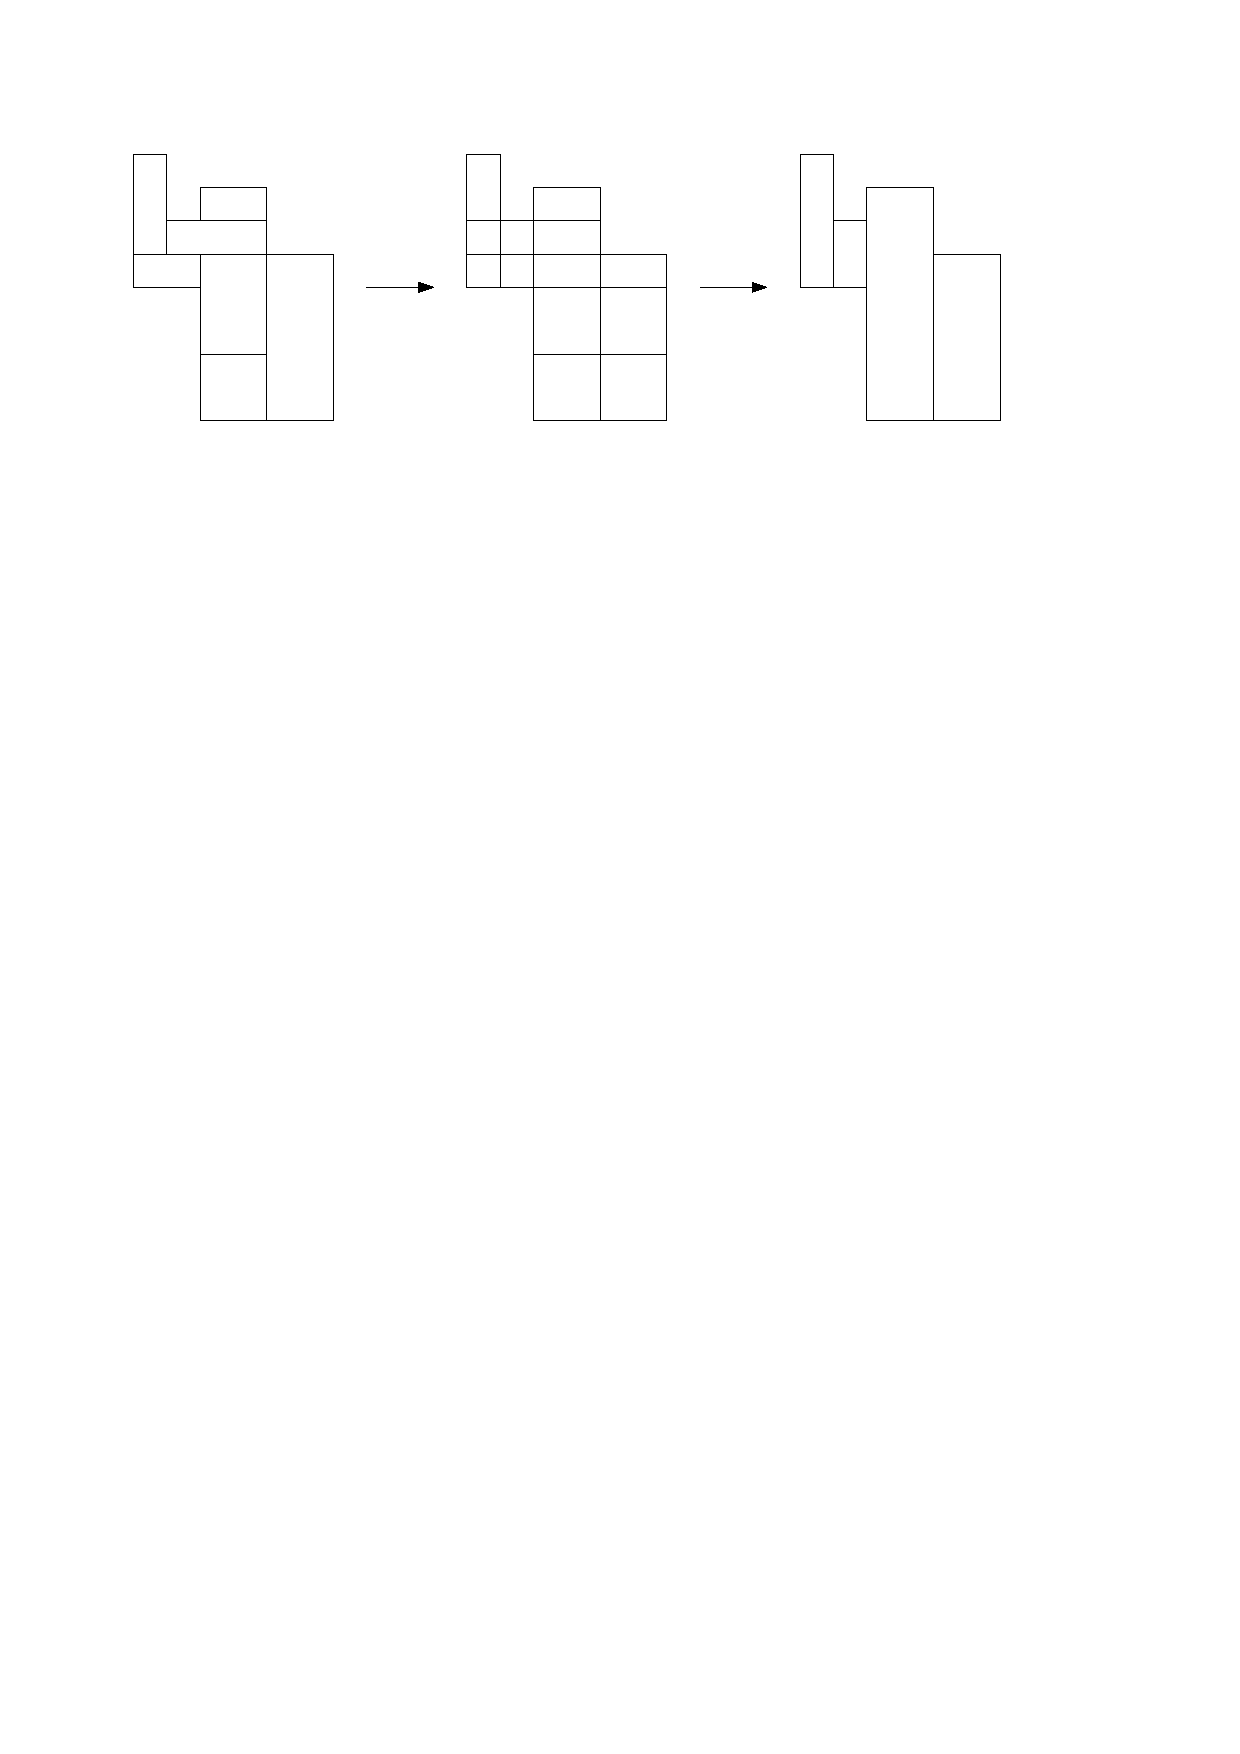
\includegraphics[scale = 0.5]{rects.pdf}
				\end{center}
			\end{figure}

			Если у нас было какое-то другое разбиение, мы получим какое-то другое разбиение на столбцы. После этого не очень трудно доказать, что два разбиения на столбцы задают одинкаовые объёмы: нужно просто нанести и те, и те линии, а после доказать, что <<суммарное>> разбиение задаёт тот же объём.

			В $n$-мерном случае нужно действовать индукцией по размерности: основания <<столбцов>> будут многомерные, а независимость от разбиения для $n-1$ будет использоваться, когда мы будем смотреть на разбиения оснований.
 		\end{proof}
	\end{st}

	\begin{thm}
		Объём~--- конечно-аддитивная функция на $\Cell_n$.
		\begin{proof}
			Теперь это очевидно: если в дизъюнктном объединении множеств из $\Cell_n$ разбить каждый элемент на ячейки, то мы получим разбиение объединения на ячейки; а в конечных суммах ассоциативность точно работает.
		\end{proof}
	\end{thm}

	\begin{thm}
		Объём~--- счётно-аддитивная функция на $\Cell_n$.
		\begin{proof}
			Переформулируем утверждение: $A, \, A_1, \, ... \in \Cell_n,$ $\sqcup A_i = A$. Доказать хочется, что
			\[
				\sum\limits_{k = 1}^{\infty} v_n(A_k) = v_n(A).
			\]
			Рассмотрим сначала частный случай: пусть $A = \Delta$ и $A_k = \Delta_k$~--- ячейки.

			\begin{enumerate}
				\item 
				Пусть $\Delta$~--- ограниченная ячейка в $\R^n, \; \varepsilon > 0$. Тогда можно взять замкнутый параллелепипед $\Delta' \subset \Delta$ и открытый $\Delta'' \supset \Delta$ такие, что
				\[
					v_n(\Delta) - v_n(\Delta') < \varepsilon \text{ и } v_n(\Delta'') - v_n(\Delta) < \varepsilon. 
				\]
				Явно они будут выглядеть, как
				\begin{align*}
					\Delta &= \prod_{k = 1}^n [a_k, \, b_k), \\
					\Delta' &= \prod_{k = 1}^n \left[a_k, \, b_k - \dfrac{1}{i}\right], \\
					\Delta'' &= \prod_{k = 1}^n \left(a_k + \dfrac{1}{i}, \, b_k\right), \\
				\end{align*}
				где $i \in \N$.

				Проделаем это для ячеек $\Delta$ и $\Delta_k\col$
				\begin{align*}
					\all \varepsilon > 0 \; \ex \Delta' \subset \Delta \col \; v_n(\Delta') &> v_n(\Delta) - \varepsilon \\ 
					\all k \; \ex \Delta_k \subset \Delta_k'' \col \; v_n(\Delta_k'') &< v_n(\Delta_k) + \dfrac{\varepsilon}{2^k}.
				\end{align*}

				Заметим, что
				\[
					\underbrace{\Delta'}_{\mathclap{\text{компакт}}} \subset \Delta = \bigsqcup\limits_{k = 1}^{\infty} \Delta_k \subset \underbrace{\bigsqcup\limits_{k = 1}^{\infty} \Delta_k''}_{\mathclap{\text{открытое покрытие}}}.
				\]
				По определению компакта 
				\[
					\Delta' \subset \bigcup_{k = 1}^{N} \Delta_k''.
				\]
				Теперь запишем объёмы:
				\[
					v_n(\Delta') \leqslant v_n\left(\bigcup_{k = 1}^{N} \Delta_k''\right) \leqslant \sum\limits_{k = 1}^{N} v_n(\Delta_k'') < \sum\limits_{k = 1}^{N} v_n(\Delta_k) + \sum\limits_{k = 1}^{N} \dfrac{\varepsilon}{2^k} < \sum\limits_{k = 1}^{N} v_n(\Delta_k) + \varepsilon.
				\]
				Используя неравенство для $v_n(\Delta')$ запишем
				\[
					v_n(\Delta) < \sum\limits_{k = 1}^{N} v_n(\Delta_k) + 2\varepsilon.
				\]
				Устремляя $\varepsilon$ к нулю и увеличивая сумму в правой части, имеем
				\[
					v_n(\Delta) \leqslant \sum\limits_{k = 1}^{\infty} v_n(\Delta_k).
				\]

				С другой стороны, 
				\[
					\bigsqcup\limits_{k = 1}^{N} \Delta_k \subset \Delta \so \sum\limits_{k = 1}^N v_n(\Delta_k) \leqslant v_n(\Delta) \so \sum\limits_{k = 1}^{\infty} v_n(\Delta_k) \leqslant v_n(\Delta).
				\]

				Поэтому на самом деле имеет место равенство.

				\item Для неограниченной ячейки интересна лишь гипотетическая ситуация, в которой $v_n(\Delta) = \infty,$ а сумма оказывается конечной (а значит, и все $\Delta_k$ ограниченные). Для неё вроде работает примерно та же оценка, что и в первом случае.
			\end{enumerate}
			Понятно, что разбивать сразу можно на ячейки, а не на элементы $\Cell_n,$ потому что каждый из них разбивается на конечное число ячеек. Чтобы $A$ тожн сделать ячейкой, нужно разбить его не конечное число ячеек, а потом немного изменить разбиения составных частей, чтобы каждая из этих ячеек разбивалась на составные ячейки составных частей. Лень.
		\end{proof}
	\end{thm}

	Поэтому объём~--- мера на алгебре $\Cell_n$.

	\begin{de}
		Мера $\mu$ на $\sigma$-алгебре $\mc{A}$ называется \ti{полной,} если для любого $A \in \mc{A}$ такого, что $\mu(A) = 0$ верно, что $\all B \subset A \; \mu(B) = 0$.
	\end{de}

	\begin{de}
		Мера на алгебре $\mc{A}$ называется \ti{$\sigma$-конечной,} если существуют $X_k$ такие, что $\mu(X_k) < \infty$ и 
		\[
			\bigcup\limits_{k = 1}^{\infty} X_k = X.
		\]
	\end{de}

	Например, уже введённый объём $v_n$~--- $\sigma$-конечная мера.

	\begin{de}
		Пусть $\mc{A}_1 \subset \mc{A}_2$~--- алгебры, и $\mu_1, \, \mu_2$~--- меры на них. Тогда $\mu_2$ называют \ti{продолжением} $\mu_1,$ если $\mu_2|_{\mc{A}_1} = \mu_1$.
	\end{de}

	\begin{thm}[Лебега-Каратеодори]
		Пусть $\mu$~--- $\sigma$-конечная мера на алгебре $\mc{A}$. Тогда:
		\begin{enumerate}
			\item Существуют её полные продолжения на $\sigma$-алгебры.
			\item Среди них есть единственное продолжение $\ov{\mu}$ такое, что если $\mu'$~--- полное продолжение $\mu,$ то $\mu'$~--- полное продолжение $\ov{\mu}$. Его называют \ti{стандартным}.
		\end{enumerate}
		\begin{proof}[Набросок доказательства]
			$\hphantom{.}$

			\begin{enumerate}
				\item
				Построим функцию $\mu^{*}\col \; 2^{X} \to [0, \, \infty]$ таким образом:
				\[
					\mu^{*}(E) = \inf \left\{\sum\limits_{k = 1}^{\infty} \mu(A_k) \bigg| \{A_k\}_{k = 1}^{\infty} \subset \mc{A}, \; \bigcup\limits_{k = 1}^{\infty} A_k \supset E \right\}.
				\]
				Она называется \ti{внешней мерой} для меры $\mu,$ но мерой не является: ей не хватает счётной аддитивности.
				\item $E \subset X$ называют \ti{хорошо разбивающим,} если $\all A \in \mc{A} \; \mu^{*}(A) = \mu^{*}(A \cap E) + \mu^{*}(A \setminus E)$. Можно доказать, что класс хорошо разбивающих множеств $\ov{\mc{A}}$ является $\sigma$-алгеброй, а $\mu^{*}$~--- мерой и является стандартным продолжением $\mu$.
			\end{enumerate}
		\end{proof}
	\end{thm}

	\begin{de}
		\ti{Мера Лебега} $\lambda_n$ на $\R^n$~--- стандартное продолжение объёма. $\sigma$-алгебра, на которой она определена, обозначается $\mc{M}_n$.
	\end{de}

	\begin{pr}
		Все борелевские множества измеримы по Лебегу.
		\begin{proof}
			$\sigma$-алгебра борелевских множеств~--- наименьшая, содержащая $\Cell_n,$ поэтому она содержится в $\mc{M}_n$.
		\end{proof}
	\end{pr}

	\begin{pr}
		Мера Лебега точки~--- ноль.
		\begin{proof}
			Это следует из того, что внешняя мера точки ноль, потому что существует сколь угодно малая ячейка, которая её содержит.
		\end{proof}
	\end{pr}

	\begin{pr}
		Конечные и счётные множества имеют нулевую меру Лебега.
		\begin{proof}
			Из-за счётной аддитивности.
		\end{proof}
	\end{pr}

	\begin{pr}
		Пусть $L \subset \R^n$~--- линейное подпространство размерности меньше, чем $n$. Тогда его мера Лебега равна нулю.
		\begin{proof}
			Нужно покрыть ячейками и сделать оценку.
		\end{proof}
	\end{pr}

	\begin{pr}(Регулярность)
		Пусть $A \in \mc{M}_n, \; \varepsilon > 0$. Тогда найдутся открытое $G$ и замкнутое $F$ такие, что 
		\[
			F \subset A \subset G, \; \lambda_n(G \setminus A) < \varepsilon, \; \lambda_n(A \setminus F) < \varepsilon. 
		\]
		\begin{proof}
			В случае, когда $E$ ограничено, это совсем просто: нужно взять покрывающий набор ячеек из определения внешней меры, и каждую ячейку приблизить открытым параллелипипедом, а потом провернуть оценку. Чтобы получить замкнутое множество, придётся повторить это для дополнения $E$ относительно какого-нибудь куба, содержащего $E$.

			Для бесконечных надо доказать!
		\end{proof}
	\end{pr}

\section{Измеримость функции относительно \texorpdfstring{$\sigma$}{σ}-алгебры. \\Свойства измеримых функций.}

	\begin{de}
		Функция $f\col \; X \to \R$ называется \ti{измеримой} относительно $\sigma$-алгебры $\mc{A},$ если для любого промежутка $\Delta \in \R \; f^{-1}(\Delta) \in \mc{A}$. 
	\end{de}

	\begin{de}
		Множества вида $X[f < a] = \{x \in X \, | \, f(x) < a\}$~--- \ti{множества Лебега $1$ типа,} а $X[f \leqslant a], \; X[f > a], \; X[f \geqslant a]$~--- $2, \; 3,$ и $4$ соответственно.  
	\end{de}

	\begin{thm}
		Чтобы функция $f$ была измерима относительно $\mc{A},$ достаточно, чтобы все множества одного из четырёх типов Лебега лежали в $\mc{A}$.
		\begin{proof}
			$\hphantom{.}$
			\begin{enumerate}
				\item $1 \to 2 \col$ 
				\[
					X[f \leqslant a] = \bigcup\limits_{k = 1}^{\infty} X\left[f < a - \dfrac{1}{k}\right].
				\] 
				\item $2 \to 3 \col \; X[f > a] = X \setminus X[f \leqslant a]$.
				\item $3 \to 4\col$ так же, как $1 \to 2$.
				\item $4 \to 1\col$ так же, как $2 \to 3$.
			\end{enumerate}
			Имея множества Лебега всех четырёх типов, нетрудно получить из них все промежутки.
		\end{proof}
	\end{thm}

	\begin{lm}
		Любое открытое множество $G \subset \R^n$ представимо, как счётное объединение ячеек.
		\begin{proof}
			Возьмём около каждой рациональной точки $G$ окрестность в форме параллелипипеда, лежащую в $G$. Понятно, что из того, что множество рациональных точек всюду плотно, следует, что мы получили счётное открытое покрытие $G$. 

			В свою очередь, любой открытый параллелипипед легко представить, как объединение счётного количества ячеек. А счётное объединение счётных объединений~--- счётное объединение.
		\end{proof}
	\end{lm}

	\begin{thm}
		Пусть функции $f_1, \, ..., \, f_n \col \; X \to \R$ измеримы, а функция $g \col \; \R^n \to \R$ непрерывна. Тогда функция $\varphi = g \circ f \col \; X \to \R$ измерима.
		\begin{proof}
			Т.к. функция $g$ непрерывна, $G = \R^n[g < a]$~--- открытое множество. Его можно представить, как
			\[
				G = \bigcup\limits_{k = 1}^{\infty} \Delta_k,
			\]
			где $\Delta_k$~--- ячейки. Тогда
			\[
				X[\varphi < a] = f^{-1}(G) = \bigcup\limits_{k = 1}^{\infty} f^{-1}(\Delta_k).
			\]
			Пусть
			\[
				\Delta_k = \prod\limits_{i = 1}^n [a_i, \, b_i).
			\]
			Тогда
			\[
				f^{-1}(\Delta_k) = \bigcap\limits_{i = 1}^{n} X[a_i \leqslant f_i < b_i].
			\]
			Поэтому
			\[
				X[\varphi < a] = \bigcup\limits_{k = 1}^{\infty} \bigcap\limits_{i = 1}^{n} X[a_i^{(k)} \leqslant f_i < b_i^{(k)}].
			\]
			Это измеримое множество.
		\end{proof}
	\end{thm}

	\begin{thm}
		$f, \, g$ измеримы $\so$ измеримы $f + g, \; f - g, \; fg, \; \tfrac{f}{g}, \; |f|, \; \lambda f, \; f \vee g = \max\{f, \, g\}, \; f \wedge g = \min\{f, \, g\}, \; f^n$.
		\begin{proof}
			Довольно очевидное следствие предыдущей теоремы.
		\end{proof}
	\end{thm}

	\begin{thm}
		Если $\{f_i\}_{i = 1}^{\infty}$ измеримы, то измеримы и $\sup f_i, \; \inf f_i, \; \underline{\lim} f_i, \; \ov{\lim} f_i, \; \lim f_i$.
		\begin{proof}
			$\hphantom{.}$
			\begin{enumerate}
				\item $g = \sup f_i \scol \; X[g \leqslant a] = X[\all i \; f_i \leqslant a] = \bigcap\limits_{i = 1}^{\infty} X[f_i \leqslant a]$.
				\item Инфимум~--- аналогично.
				\item $g = \lim f_i \so \left(g(x) \leqslant a \eqv \ex N \col \; \all i > N \; f_i(x) \leqslant a\right) \so X[g \leqslant a] = \bigcup\limits_{N = 1}^{\infty} \bigcap\limits_{i = N + 1}^{\infty} X[f_i(x) \leqslant a]$.
				\item Верхний и нижний пределы~--- пределы инфимумов и супремумов, поэтому эти результаты следуют из уже доказанного.
			\end{enumerate}
		\end{proof}
	\end{thm}

	\begin{de}
		$f \col \; X \to \R$ называется \ti{простой} (относительно $\mc{A}$,) если она измерима относительно $\mc{A}$ и принимает конечное число значений.
	\end{de}

	\begin{de}
		\ti{Индикатором} множества $E$ называется функция 
		\[
			\mathbb{1}_E(x) = \begin{cases}
				1, \; x \in E, \\
				0, \; x \notin E.
			\end{cases}
		\]
	\end{de}

	\begin{st}
		Индикатор $E$ прост (измерим) тогда и только тогда, когда измеримо $E$.
	\end{st}

	\begin{st}
		Пусть $f$~--- функция, которая принимает значения $\{a_i\}_{i = 1}^{N}$ на множествах $E_i$. Тогда
		\[
			f = \sum\limits_{i = 1}^N a_i \mathbb{1}_{f^{-1}(a_i)} = \sum\limits_{i = 1}^N a_i \mathbb{1}_{E_i}.
		\]
	\end{st}

	\begin{st}
		Функция $f$, принимающая конечное число значений, проста (измерима) тогда и только тогда, когда множества $E_i$ измеримы.
	\end{st}

	\begin{thm}
		Если $\{f_i\}_{i = 1}^{\infty}$~--- последовательность простых функций, имеющая предел, то этот предел измерим.
	\end{thm}

	\begin{thm}
		Пусть $f$~--- неотрицательная измеримая функция. Тогда найдётся неубывающая последовательность $\{\varphi_i\}_{i = 1}^{\infty}$ простых функций, которая поточечно сходится к $f$.
		\begin{proof}
			Разобъём $[0, +\infty)$ следующим образом:
			\[
				[0, \infty) = \bigsqcup\limits_{k = 0}^{n^2} \Delta_k,
			\]
			где
			\[
				\Delta_k = \begin{cases}
					\left[\dfrac{k}{n}, \, \dfrac{k + 1}{n}\right], \; 0 \leqslant k < n^2, \vspace{0.5em}\\
					[n, \, \infty), \; k = n^2.
				\end{cases}
			\]

			Пусть $e_k = f^{-1}(\Delta_k) \in \mc{A}, \; c_k = \min \Delta_k = \dfrac{k}{n}$ и
			\[
				\psi_n = \sum\limits_{k = 0}^{n^2} c_k \mathbb{1}_{e_k}.
			\]

			Рассмотрим $x \in e_k$. Начиная с некоторого $n$ эта точка точно попадёт в $e_k$ с $k < n^2$. Значение $f(x) \in \Delta_k = \left[c_k, \, c_k + \dfrac{1}{n}\right],$ поэтому 
			\[
				|f(x) - \psi_n(x)| \leqslant \dfrac{1}{n}
			\]
			начиная с некоторого $n$. Отсюда следует поточечная сходимость.

			Чтобы сделать последовательность функций неубывающей, сохранив сходимость, введём
			\[
				\varphi_n = \max\{\psi_1, \, ..., \, \psi_n\}.
			\]
			Сходимость сохранится, т.к.
			\[
				f - \dfrac{1}{n} \leqslant \psi_n \leqslant \varphi_n \leqslant f. 
			\]
		\end{proof}
	\end{thm}

\section{Определение интеграла по мере. Свойства интеграла от неотрицательных функций.}
	
	\begin{de}
		Пусть $f$~--- простая, и представлена, как
		\[
			\sum\limits_{k = 1}^p c_k \mathbb{1}_{E_k}.
		\]
		Тогда
		\[
			\int\limits_{X} f \D \mu = \sum\limits_{k = 1}^p c_k \, \mu(E_k).
		\]
		Если $A \in \mc{A},$ то
		\[
			\int\limits_{A} f \D \mu = \sum\limits_{k = 1}^p c_k \, \mu(E_k \cap A).
		\]
	\end{de}

	\begin{st}
		Если $f$~--- простая на $X,$ то 
		\[
			\int\limits_{A} f \D \mu = \int\limits_{X} f \, \mathbb{1}_A \D \mu.
		\]
		\begin{proof}
			\[
				f \, \mathbb{1}_A = \mathbb{1}_A \sum\limits_{k = 1}^p c_k \mathbb{1}_{E_k} = \sum\limits_{k = 1}^p c_k \mathbb{1}_{E_k \cap A}. 
			\]
		\end{proof}
	\end{st}

	\begin{de}
		Пусть $f$~--- измеримая, неотрицательная функция. Тогда
		\[
			\int\limits_{X} f \D \mu = \sup \left\{\,\int\limits_{X} g \D \mu \, \bigg|\, g\text{~--- простая}, \; 0 \leqslant g \leqslant f \right\}
		\]
		При этом
		\[
			\int\limits_{A} f \D \mu = \int\limits_{X} f \, \mathbb{1}_A \D \mu.
		\]
	\end{de}

	В следующих свойствах функции измеримые и неотрицательные.

	\begin{pr}
		\[
			0 \leqslant f \leqslant g \so  \int\limits_{X} f \D \mu \leqslant \int\limits_{X} g \D \mu. 
		\]
		\begin{proof}
			Очевидно из определения, для $g$ супремум берётся по большему множеству функций.
		\end{proof}
	\end{pr}

	\begin{pr}
		\[
			A \subset B \subset X \so \int\limits_{B} f \D \mu \leqslant \int\limits_{A} f \D \mu. 
		\]
		\begin{proof}
				Следует из предыдущего свойства.
		\end{proof}
	\end{pr}

	\begin{de}
		Пусть $f$~--- произвольная измеримая функция. Определим
		\[
			f_{+} = \max\{f(x), \, 0\}, \; f_{-} = \max\{-f(x), \, 0\}.
		\]
		Тогда
		\[
			\int\limits_{X} f \D \mu = \int\limits_{X} f_{+} \D \mu - \int\limits_{X} f_{-} \D \mu.
		\]
	\end{de}

	\begin{de}
		$f$ называется \ti{суммируемой} на $X,$ если интеграл от неё конечен. Семейство суммируемых функций обозначается, как $L(X, \, \mu)$.
	\end{de}

\section{Теорема Беппо Леви.}
	
	\begin{thm}
		Пусть $\{f_n\}_{n = 1}^{\infty}$~--- неубывающая последовательность измеримых неотрицательных функций, и $f = \lim f_n$. Тогда
		\[
			\int\limits_{X} f \D \mu = \lim \int\limits_{X} f_n \D \mu.
		\]
		\begin{proof}
			\begin{align*}
				f_n \leqslant f \so& \int\limits_{X} f_n \D \mu \leqslant \int\limits_{X} f \D \mu, \\
				f_n \leqslant f_{n + 1} \so& \int\limits_{X} f_n \D \mu \leqslant \int\limits_{X} f_{n+1} \D \mu \so \ex \lim \int\limits_{X} f_n \D \mu = L.
			\end{align*}
			Из этих двух утверждений следует, что
			\[
				L \leqslant \int\limits_{X} f \D \mu.
			\]

			Теперь проверим неравенство в другую сторону. По определению
			\[
				\int\limits_{X} f \D \mu = \sup\limits_{\varphi} \int\limits_{X} \varphi \D \mu,
			\]
			где $\varphi$~--- неотрицательные простые функции, не превосходящие $f$. Рассмотрим какую-нибудь $\varphi\col$
			\[
				\varphi = \sum\limits_{k = 1}^p c_k \mathbb{1}_{E_k},
			\]
			причём $c_k \geqslant 0$. Примем $c_0 = 0\scol$ тогда понятно, что $E_0 = \varnothing \eqv \varphi > 0$.

			Возьмём $\varepsilon\col \; 0 < \varepsilon < \min\{c_1, \, ..., \, c_p\}$ и 
			\[
				\varphi_{\varepsilon} = 0 \cdot \mathbb{1}_{E_0} + \sum\limits_{k = 1}^p (c_k - \varepsilon) \mathbb{1}_{E_k}.
			\]
			Рассмотрим $X_n = X[f_n \geqslant \varphi_{\varepsilon}]$. Понятно, что $E_0 \subset X_n$.

			Т.к. $f_n \to f,$ для любой точки $x$ найдётся $n$ такое, что $f_n(x) > \varphi_{\varepsilon}(x),$ т.е. 
			\[
				\all x \; \ex n \col \; x \in X_n.
			\]
			Поэтому
			\[
				\bigcup\limits_{n = 1}^{\infty} X_n = X.
			\]
			Т.к. последовательность неубывающая, $X_n \subset X_{n + 1} \so \mu(X_n) \xrightarrow{n \to \infty}\mu(X)$. Вообще, для любого измеримого $A$ верно, что $\mu(A \cap X_n) \xrightarrow{n \to \infty}\mu(A)$.

			\[
				\int\limits_{X} f_n \D \mu \geqslant \int\limits_{X_n} f_n \D \mu \geqslant \int\limits_{X_n} \varphi_{\varepsilon} \D \mu = \sum\limits_{k = 1}^p (c_k - \varepsilon) \, \mu(X_n \cap E_k). 
			\]
			Устремляя $n$ к бесконечности и $\varepsilon$ к нулю, получим
			\[
				L \geqslant \sum\limits_{k = 1}^p c_k \, \mu(E_k) = \int\limits_{X} \varphi \D \mu.
			\]
			Переходя к супремуму, получим
			\[
				L \geqslant \int\limits_{X} f \D \mu.
			\]
			Значит, на самом деле есть равенство.
		\end{proof}
	\end{thm}

	\begin{pr}
		Пусть $f, g$~--- измеримые и неотрицательные функции. Тогда
		\[
			\int\limits_{X} (f + g) \D \mu = \int\limits_{X} f \D \mu + \int\limits_{X} g \D \mu.
		\]
		\begin{proof}
			Нужно сначала проверить для простых функций, записав их через индикаторы и повозившись с суммами. После этого в общем случае можно выделить возрастающие последовательности простых функций, которые сходятся к $f$ и $g$ и воспользоваться теоремой Леви.
		\end{proof}
	\end{pr}

	\begin{pr}
		\[
			\int\limits_{X} \lambda f \D \mu = \lambda \int\limits_{X} f \D \mu.
		\]
		\begin{proof}
			Аналогично.
		\end{proof}
	\end{pr}

\section{Свойства интеграла от суммируемых функций.}
	
	\begin{pr}
		Пусть $f, \, g$~--- суммируемые, $f \leqslant g$. Тогда
		\[
			\int\limits_{X} f \D \mu \leqslant \int\limits_{X} g \D \mu.
		\]
		\begin{proof}
			Расписать положительную и отрицательную части и свести к свойству для неотрицательных функций; суммируемость нужна, чтобы не вычитать бесконечность из неравенства.
		\end{proof}
	\end{pr}

	\begin{pr}\footnote{В конспекте был $\pm,$ но это ведь следует из умножения на константу? И, кстати, нужна ли тут вообще суммируемость, или это верно, даже когда интеграл расходится?}
		Пусть $f, \, g$~--- суммируемые. Тогда
		\[
			\int\limits_{X} f + g \D \mu \leqslant \int\limits_{X} f \D \mu + \int\limits_{X} g \D \mu.
		\]
		\begin{proof}
			Аналогично.
		\end{proof}
	\end{pr}

	\begin{pr}
		Если $f$~--- суммируемая, то
		\[
			\int\limits_{X} \lambda f \D \mu = \lambda \int\limits_{X} f \D \mu.
		\]
		\begin{proof}
			Аналогично.
		\end{proof}
	\end{pr}

	\begin{pr}
		Пусть $f, \, g \in L, \; |f| \leqslant g \so \left|\int f \right| \leqslant \int g$. 
		\begin{proof}
			\[
				|f| \leqslant g \so f \leqslant g \wedge -f \leqslant g \so \left(\int f \leqslant \int g \right) \wedge \left(-\int f \leqslant \int g\right) \so \left| \int f \right| \leqslant \int g.
			\]
		\end{proof}
	\end{pr}

	\begin{pr}
		$\left|\int f\right| \leqslant \int |f|$.
		\begin{proof}
			Очевидно следует из предыдущего.
		\end{proof}
	\end{pr}

	\begin{pr}
		$f \in L \eqv |f| \in L$.
		\begin{proof}
			$\bso\col$ 
			\[
				|f| = f_{+} + f_{-} \so 0 \leqslant f_{\pm} \leqslant |f| \so 0 \leqslant \int f_{\pm} \leqslant \int |f|.
			\] 
			$\so\col$ Если $f$ суммируема, то суммируемы и $f_{\pm},$ а $|f|$~--- их сумма.
		\end{proof}
	\end{pr}

	\begin{pr}
		$f \in L,$ $\mu X \leqslant \infty, \; |f|\leqslant M \so \left|\int f \D \mu\right| \leqslant M \mu(X)$.
		\begin{proof}
			\[
				\left|\int f \D \mu\right| \leqslant \int |f| \D \mu \leqslant \int M \D \mu \leqslant M \mu(X). 
			\]
		\end{proof}
	\end{pr}

\section{Счётная аддитивность интеграла.}

	\begin{thm}
		Пусть $f$~--- измеримая функция, причём либо $f \geqslant 0,$ либо $f \in L$. Тогда для любых измеримых $A, \, A_1, \, ...$ таких, что $A = \sqcup A_k$ верно, что
		\[
			\int\limits_{A} f = \sum\limits_{k = 1}^{\infty} \, \int\limits_{A_k} f.
		\]
		\begin{proof}
			$\hphantom{.}$
			\begin{enumerate}
				\item Пусть $f \geqslant 0$. Тогда
				\[
					\int\limits_{A} f = \int\limits_{X} f \, \mathbb{1}_{A}, \; \int\limits_{A_n} f = \int\limits_{X} f \, \mathbb{1}_{A_n}.
				\]
				При этом
				\[
					\sum\limits_{n = 1}^{\infty} \mathbb{1}_{A_n} = \mathbb{1}_A \so f \, \mathbb{1}_{A} = \sum\limits_{n = 1}^{\infty} f \, \mathbb{1}_{A_n}
				\]

				Рассмотрим частичные суммы:
				\[
					S_N = \sum\limits_{n = 1}^{N} f \, \mathbb{1}_{A_n}.
				\]
				Понятно, что они образуют неубывающую неотрицательную последовательность, сходящуюся к $f \, \mathbb{1}_{A},$ поэтому из теоремы Леви
				\[
					\int f \, \mathbb{1}_{A} = \lim \int S_n = \lim \int \sum\limits_{n = 1}^{N} f \, \mathbb{1}_{A_n} = \lim \sum\limits_{n = 1}^{N} \, \int\limits_{A_n} f = \sum\limits_{n = 1}^{\infty} \, \int\limits_{A_n} f.
				\]
				\item Пусть теперь $f \in L$. Тогда просто расписать через $f_{\pm}$ и воспользоваться первым пунктом.
			\end{enumerate}
		\end{proof}
	\end{thm}

\section{Абсолютная неперывность интеграла}

	\begin{thm}
		Пусть $f \in L$. Тогда
		\[
			\all \varepsilon > 0 \; \ex \delta > 0 \col \; \all \text{ измеримого } A \subset X, \; \mu(A) < \delta \so \left|\int\limits_{A} f \D \mu\right| < \varepsilon. 
		\]
		\begin{proof}
			$\hphantom{.}$
			\begin{enumerate}
				\item
				Если $f$ ограничена, то найдётся $M$ такое, что $|f| \leqslant M$. Тогда 
				\[
					\left|\int\limits_{A} f \right| \leqslant M \mu(A) \leqslant \varepsilon \text{ при } \delta = \dfrac{\varepsilon}{M}.
				\]
				\item Пусть теперь $f \in L$ и всё. Тогда $|f| \in L,$ и 
				\[
					\int\limits_X |f| = \sup\limits_g \int\limits_X g.
				\]
				$g$~--- простая, а потому ограниченная.
				\[
					\all \varepsilon > 0 \, \ex \text{ простая } g, \; 0 \leqslant g \leqslant |f| \col \; \int\limits_X |f| - \int\limits_X g < \dfrac{\varepsilon}{2}.
				\]

				Используя ограниченность $g,$ находим по любому $\varepsilon$ такую $\delta,$ что
				\[
					\mu(A) < \delta \so \int\limits_A g < \dfrac{\varepsilon}{2}. 
				\]

				Отсюда мгновенно получается искомая оценка:
				\[
					\left|\int\limits_{A} f\right| \leqslant \int\limits_{A} |f| = \int\limits_{A} g + \int\limits_{A} \big(|f| - g\big) < \varepsilon.	 	
				\]
			\end{enumerate}
		\end{proof}
	\end{thm}

\section{Вычисление интеграла от непрерывной функции по мере Лебега.}

	\begin{thm}
		Пусть $f \in C([a, \, b])$ и $\lambda$~--- мера Лебега. Тогда $f$ суммируема и 
		\[
			\int\limits_{[a, \, b]} f \D \lambda = \int\limits_a^b f.
		\]
		\begin{proof}
			$\hphantom{.}$
			\begin{enumerate}
				\item Сначала докажем, что $f$ измерима по Лебегу. Заметим, что $f^{-1}\big((-\infty, \, a)\big)$~--- открытое множество, т.е. измеримое множество. А значит и функция $f$ измерима.
				\item $|f|$ ограничен, т.к. $f$~--- непрерывная функция на компакте, поэтому
				\[
					\int\limits_{[a, \, b]} |f| \D \lambda \leqslant \int\limits_{[a, \, b]} M \D \lambda \leqslant M(b - a).
				\]
				Значит, $|f|$~--- суммируемая функция, а значит, и $f$~--- суммируемая функция. 
				\item Рассмотрим функцию
				\[
					F(x) = \int\limits_{[a, \, x]} f \D \lambda.
				\]
				Она определена, поскольку все интегралы будут конечны. Хочется доказать, что она дифференцируема.

				Запишем, что значит непрерывность функции:
				\[
					\all \varepsilon > 0 \; \ex \delta \col \; |\Delta x| < \delta \so \all t \in (x - \Delta x, \, x + \Delta x) \; f(t) \in (f(x) - \varepsilon, \, f(x) + \varepsilon).
				\]
				Отсюда следует, что
				\[
					\Delta x \, (f(x) - \varepsilon) \leqslant \int\limits_{\mathclap{(x, \, x + \Delta x]}} f \D \lambda \leqslant \Delta x \, (f(x) + \varepsilon).
				\]
				Разделив на $\Delta x$ и подставив интеграл посередине, получаем, что
				\[
					\all \varepsilon > 0 \; \ex \delta \col \; |\Delta x| < \delta \so \left|\dfrac{F(x + \Delta x) - F(x)}{\Delta x} - f(x)\right| < \varepsilon.
				\]
				Но это значит, что $F'(x) = f(x)!$ Поэтому значение нашего интеграла будет такое же, как по Риману.
			\end{enumerate}
		\end{proof}
	\end{thm}

\section{Сравнение подходов Римана и Лебега}
	
	Есть три разных способа определить интеграл на отрезке:

	\begin{enumerate}
		\item (подход Ньютона-Лейбница) Если $f$ непрерывна и $F$~--- её первообразная, то
		\[
			\int\limits_a^b f(x) \D x = F(b) - F(a),
		\]
		\item (подход Римана)
		\[
			\int\limits_a^b f(x) \D x = \lim\limits_{\max\{\Delta x_i\} \to 0} \sum\limits_{i = 0}^{n + 1} f(\xi_i) \Delta x_i, \; \xi_i \in [x_i, \, x_{i + 1}], \; \Delta x_i = x_{i + 1} - x_i.
		\]
		\item Наше текущее определение интеграла по мере.
	\end{enumerate}

	\begin{exm}
		Функция Дирихле $f\col \; X = [0, \, 1] \to \R\col$
		\[
			f(x) = \begin{cases}
				1, \; x \in \Q, \\
				0, \; x \notin \Q.
			\end{cases}
		\]
		Интеграл по Риману от неё не существует, потому что при сколь угодно малом ранге разбиения можно выбрать в каждом промежутке все $\xi_i$ рациональными, и тогда значение суммы Римана будет равно длине отрезка, или иррациональными, и тогда значение суммы будет равно нулю. Поэтому предела этих сумм при ранге разбиения, стремящемся к нулю, не существует.

		При этом $f$ является простой функцией: она принимает два значения, при этом одно из них~--- на счётном (а значит, измеримом) множестве точек. Поэтому и его дополнение тоже измеримо~--- его мера равна $1$. Поэтому интеграл Лебега от этой функции будет равен $0$.

		В суммировании по Риману основной принцип~--- разбить промежуток интегрирования на малые участки. В суммировании по Лебегу, напротив, на промежутки бьётся область значений, а промежуток интегрирования оказывается разбит на множества произвольной формы. Вид этой конструкции для интеграла Лебега подробно продемонстрирован в билете $6,$ в доказательстве теоремы о существовании сходящейся последовательности из простых функций.
	\end{exm}

\section{Сравнение интеграла по мере с несобственным интегралом}

	\begin{de}[Напоминание]
		Пусть $f$ непрерывна на $[a, \, b)$. Тогда \ti{несобственный интеграл} по этому промежутку~---
		\[
			\int\limits_a^{\to b} f = \lim\limits_{x \to b-0} \int\limits_a^{x} f.
		\]
	\end{de}

	\begin{thm}
		Пусть непрерывная $f$ либо неотрицательна, либо суммируема на $[a, \, b),$ тогда
		\[
			\int\limits_{[a, \, b)} f\D \lambda = \int\limits_a^{\to b} f.
		\]
		\begin{proof}
			Рассмотрим 
			\[
				F(x) = \int\limits_{[a, \, x]} f.
			\]
			Понятно, что\footnote{Если этот предел существует.}
			\[
				\lim\limits_{x \to b} F(x) = \int\limits_a^{\to b} f,
			\]
			потому что мы уже доказали, что интегралы по отрезку от непрерывной функции по Лебегу и по Риману совпадают.

			Нужно доказать, что
			\[
				\lim\limits_{x \to b} F(x) = \int\limits_{[a, \, b)} f.
			\]
			Если $f$ суммируема, то это следует из теоремы об абсолютной непрерывности интеграла Лебега (и существование предела оказывается совсем очевидным).

			Рассмотрим случай, когда $f$ неотрицательна, но не суммируема. Мы знаем, что интеграл Лебега от неё по $[a, \, b)$ равен $+\infty,$ и нужно лишь доказать, что предел $F(x)$ существует и не может быть конечен. Существует он потому, что $F(x)$ будет функцией возрастающей. Конечным же он быть не может, потому что это противоречило бы теореме Леви, что сейчас и покажем.

			Возьмём последовательность точек $\{x_n\}_{n = 1}^{\infty}$ из $[a, \, b),$ сходящуюся к $b$. Заметим, что
			\[
				\lim \int\limits_{[a, \, x_n]} f \D \lambda = \lim \int\limits_{[a, \, b)} f \, \mathbb{1}_{[a, \, x_n]} \D \lambda.
			\] 
			Функции $f \, \mathbb{1}_{[a, \, x_n]}$ образуют неубывющую неотрицательную последовательность, сходящуюся к $f,$ поэтому по теореме Леви этот предел будет равен как раз $+\infty$.
		\end{proof}
	\end{thm}

	\begin{exm}
		Условно сходящийся интеграл
		\[
			\int\limits_{0}^{\infty} \dfrac{\sin x}{x} \D x
		\]
		не представим в виде интеграла по мере, потому что для этой функции этот интеграл просто не определён: $f_{+}$ и $f_{-}$ одновременно не являются суммируемыми, что плохо.
	\end{exm}

\section{Интеграл по дискретной мере и по мере, задаваемой плотностью}

	\begin{de}
		Пусть $X$~--- множество, $\mc{A} = 2^{X}$ и есть не более чем счётные множества $\{a_i\} \in X$ и $\{m_i\} \in \R$. Тогда \ti{дискретная мера} задаётся, как
		\[
			\mu(E) = \sum\limits_{i} m_i \delta_{a_i}(E).
		\]
	\end{de}

	\begin{lm}
		Интеграл от любой (измеримой) функции по множеству $E$ нулевой меры равен нулю.
		\begin{proof}
			Для начала можно заметить, что для простых функций это точно так. Действительно, пусть
			\[
				f = \sum\limits_{k = 1}^p a_k \mathbb{1}_{E_k}.
			\]
			Тогда
			\[
				\int\limits_{E} \sum\limits_{k = 1}^p a_k \mathbb{1}_{E_k} = \sum\limits_{k = 1}^p a_k \int\limits_{X} \underbrace{\mathbb{1}_{E_k \cap E}}_{=0} = 0.
			\]

			Но тогда понятно, что для неотрицательных функций это тоже будет верно, потому что супремум нулей ноль. Ещё более очевидно, что для произвольных измеримых функций ничего не изменится.
		\end{proof}
	\end{lm}

	\begin{lm}
		Интеграл от измеримой функции $f$ по множеству ${a}$ равен $f(a) \mu\big(\{a\}\big)$.
		\begin{proof}
			\[
				\int\limits_{\{a\}} f = \int\limits_{X} f \, \mathbb{1}_{\{a\}} = \int\limits_{X} f(a) \, \mathbb{1}_{\{a\}} = f(a) \int\limits_{X} \mathbb{1}_{\{a\}} = f(a) \, \mu(\{a\}).
			\]
		\end{proof}
	\end{lm}

	\begin{thm}
		Пусть $f\col \; X \to \R$ либо неотрицательна, либо суммируема относительно дискретной меры. Тогда
		\[
			\int\limits_{X} f \D \mu = \sum\limits_k f(a_k) m_k.
		\]
		\begin{proof}
			Во-первых понятно, что относительно дискретной меры все функции измеримы. Во-вторых, если $E = X \setminus \{a_k\},$ можно записать
			\[
				\int\limits_{X} f \D \mu = \int\limits_{E} f \D \mu + \sum\limits_{k} \int\limits_{\{a_k\}} f \D \mu = \sum\limits_k f(a_k) m_k.
			\]
			Неотрицательность или суммируемость использовалась для счётной аддитивности.
		\end{proof}
	\end{thm}

	\begin{st}
		Для дискретной меры суммируемость функции равносильна абсолютной сходимости ряда, записанного в предыдущей теореме.
		\begin{proof}
			Суммируемость функции равносильна суммируемости её модуля. Модуль же функция неотрицательная, для него выполняется предыдущая теорема, и интеграл от него равен сумме из модулей. Значит, и их сходимости равносильны.
		\end{proof}
	\end{st}

	\begin{exm}
		Если, например, взять $X = \N, \; a_k = k$ и $m_k = 1,$ то мера будет обозначать просто сумму значений функции в точках. Функция из $\N$ в $\R$~--- ряд, а суммируемость~--- абсолютная сходимость. 
	\end{exm}

	\begin{de}
		Пусть $X$~--- пространство с мерой $\mu,$ и есть измеримая неотрицательная функция $\rho\col \; X \to \R$. Тогда можно ввести меру
		\[
			\nu(E) = \int\limits_{E} \rho \D \mu.
		\]
	\end{de}

	\begin{st}
		$\nu$ и правда мера.
		\begin{proof}
			Первая аксиома очевидна, а вторая следует из теоремы о счётной аддитивности интеграла~--- ведь наша $\rho$ неотрицательна.
		\end{proof}
	\end{st}

	\begin{thm}
		Пусть $f$ измерима на $X$ и либо неотрицательна, либо суммируема относительно $\nu$. Тогда
		\[
			\int\limits_{X} f \D \nu = \int\limits_{X} f \rho \D \mu. 
		\]
		\begin{proof}
			$\hphantom{.}$
			\begin{enumerate}
				\item Пусть сначала $f$~--- простая:
				\[
					f = \sum\limits_{k = 1}^p a_k \mathbb{1}_{E_k}.
				\]
				Тогда
				\[
					\int\limits_{X} f \D \nu = \sum\limits_{k = 1}^p a_k \nu(E_k) = \sum\limits_{k = 1}^p a_k \int\limits_{E_k} \rho \D \mu = \sum\limits_{k = 1}^p a_k \int\limits_{X} \mathbb{1}_{E_k} \, \rho \D \mu = \int\limits_{X} f \rho \D \mu.
				\]
				\item Если $f$~--- измеримая неотрицательная, можно выделить неубывающую неотрицательную последовательность простых, сходящуюся к ней. От умножения на $g$ она этих свойств не потеряет, поэтому равенство благополучно перенесётся по теореме Леви.
				\item Ну и для произвольной суммируемой нужно просто написать.
			\end{enumerate}
		\end{proof}
	\end{thm}

	\begin{de}
		$\rho$ называют \ti{плотностью} меры $\nu$ относительно меры $\mu$.
	\end{de}

	\begin{exm}
		Например, \ti{мера Коши} c 
		\[
			\rho = \dfrac{1}{1 + x^2}.
		\]
	\end{exm}

\section{Интеграл по мере Лебега-Стилтьеса. Интеграл по распределению.}
	
\subsection{Интеграл по мере Лебега-Стилтьеса.}
	\begin{de}
		Пусть $I$~--- интервал на прямой, $F \col \; I \to \R$~--- возрастающая, непрерывная слева ($F(x) = F(x - 0)$) функция. Введём функцию
		\[
			\mu\left([a, b)\right) = F(b) - F(a).
		\]
		Она счётно-аддитивна на $\Cell_1$\footnote{Кажется, это делается примерно так же, как с обычным объёмом. Но вообще там тоже было не очень строго, да и как-то грустно это.} Стандартное продолжение этой функции на $\sigma$-алгебру называется \ti{мерой Лебега-Стилтьеса}.
	\end{de}

	\begin{st}
		Все борелевсекие множества измеримы по Лебегу-Стилтьесу.
		\begin{proof}
			Рассуждение одинаково для всех мер, распространённых с ячеек.
		\end{proof}
	\end{st}

	\begin{pr}
		Пусть $\Delta = [a, \, b]$. Тогда $\mu(\Delta) = F(b + 0) - F(a)$.
		\begin{proof}
			Нужно рассмотреть сходящуюся к отрезку справа последовательность ячеек.
		\end{proof}
	\end{pr}

	\begin{pr}
		$\mu\big(\{a\}\big) = f(a + 0) - f(a) = f(a + 0) - f(a - 0) = \Delta f_a$.
	\end{pr}

	\begin{pr}
		$\mu\big((a, \, b)\big) = f(b) - f(a + 0)$.
	\end{pr}

	\begin{st}
		Любая мера, определённая на борелевских множествах, есть мера Лебега-Стилтьеса для некоторой $F$.
		\begin{proof}
			Это выглядит довольно логичным, но на паре доказательства не было.
		\end{proof}
	\end{st}

	\begin{st}
		Если $F$~--- гладкая на $I,$ и $\Delta \subset I$~--- ячейка, то
		\[
			\mu_F(\Delta) = \int\limits_{\Delta} F' \D \lambda.
		\]
		\begin{proof}
			Очевидно.
		\end{proof}
	\end{st}

	\begin{st}
		Это верно не только для ячеек, но и для множеств произвольной формы. На самом деле, в такой ситуации мера по сути задаётся плотностью $F'$.
	\end{st}

	\begin{thm}
		Пусть $F$~--- кусочно-гладкая (и обладает остальным, чтобы задать меру) на $I,$ т.е. найдутся $c_i \in I$ такие, что $F$ гладкая на $(c_i, \, c_{i+1})$. Пусть $f$ измерима (относительно борелевской алгебры $\mc{B}$) и либо суммируема относительно $\mu_F,$ либо неотрицательна. Тогда
		\[
			\int\limits_{I} f \D \mu_F = \sum \int\limits_{c_i}^{c_{i + 1}} f(x) F'(x) \D x + \sum f(c_i) \Delta_{c_i}.
		\]
		\begin{proof}
			Надо $I$ разбить на точки $c_i$ и промежутки между ними. Интеграл по точкам выражается через скачки, потому что мы знаем, что интеграл в точке равен произведению значения $f$ на меру точки. Ну а на интервалах мера по сути задаётся плотностью: про такое мы уже всё знаем.
		\end{proof}
 	\end{thm}

 \subsection{Интеграл по образу меры}
 	\begin{de}
 		Пусть $X$~--- пространство с мерой, и есть $f \col \; X \to Y$. Назовём $E \subset Y$ \ti{измеримым относительно $f$,} если $f^{-1}(E)$ измеримо.
 	\end{de}

 	\begin{st}
 		Множество измеримых относительно $f$ множеств образует $\sigma$-алгебру.
 		\begin{proof}
 			Нужно просто проверить это.
 		\end{proof}
 	\end{st}

 	\begin{de}
 		Введём меру $\nu$ на $Y$ следующим образом: $\nu(E) = \mu(f^{-1}(E))$.
 	\end{de}

 	\begin{st}
 		$\nu$ действительно мера.
 		\begin{proof}
 			Просто проверить.
 		\end{proof}
 	\end{st}

 	\begin{thm}
 		Пусть $g$~--- измеримая относительно заданной $f$ $\sigma$-алгебры функция $Y \to \R,$ причём либо неотрицательная, либо суммируемая относительно $\nu$. Тогда
 		\[
 			\int\limits_{Y} g \D \nu = \int\limits_{X} g \circ f \D \mu.
 		\]
 		\begin{proof}
 			$\hphantom{.}$
 			\begin{enumerate}
 				\item Для простых функций проверяется легко: там будет сумма коэффициентов, умноженных на меры множеств, вот эти меры и нужно раскрыть.
 				\item Если $g$ неотрицательна, то можно взять неубывающую последовательность неотрицательных простых, сходящуюся к $g$. Т.к. композиция с $g$ этого свойства не испортит, дальше просто теорема Леви.
 				\item Для суммируемых тоже как обычно: нужно просто написать $g_{\pm}$.
 			\end{enumerate}
 		\end{proof}
 	\end{thm}

 \subsection{Интеграл по распределению.}

 	\begin{de}
 		\ti{Распределением} измеримой функции $f \col \; X \to \R, \; \mu(X) < \infty$ называется 
 		\[
 			F(t) = \mu\big(X[f < t]\big).
 		\]
 	\end{de}

 	\begin{pr}
 		$F$ не убывает.
 		\begin{proof}
 			Это следует из того, что мера подмножества не превосходит меры множества.
 		\end{proof}
 	\end{pr}

 	\begin{pr}
 		$F$ непрерывна слева.
 		\begin{proof}
 			Следует из непрерывности меры снизу.
 		\end{proof}
 	\end{pr}

 	\begin{thm}
 		Пусть $\mu(X) < \infty, \; f\col\; X \to \R$ измерима и либо неотрицательна, либо суммируема. Тогда
 		\[
 			\int\limits_{X} f \D \mu = \int\limits_{\R} t \D \mu_{F}.
 		\]
 		\begin{proof}
 			Убедимся, что $\mu_F = \nu = \mu \circ f^{-1},$ как в теореме про образ меры. Для ячеек это проверяется тривиально:
 			\[
 				\mu_F \big([a, \, b)\big) = F(b) - F(a) = \mu\big(X[f < b]\big) - \mu\big(X[f < a]\big) = \mu \big(X[a \leqslant f < b]\big) = \mu\big(f^{-1}([a, \, b)\big).
 			\]
 			Отсюда это вроде бы следует даже для борелевских множеств.

 			Но тогда
 			\[
 				\int\limits_{\R} t \D \mu_{F} = \int\limits_{X} f \D \mu.
 			\]
 			Конечность меры $X$ нужна, чтобы $F$ гарантированно существовала. В принципе, такое бывает и без неё.
 		\end{proof}
 	\end{thm}

\section{Интеграл Эйлера-Пуассона}

	\begin{thm}
		\[
			\int\limits_{\R^2} e^{-(x^2 + y^2)} \D \lambda_2 = \pi.
		\]
		\begin{proof}
			Найдём распределение функции $f(x, \, y) = -e^{-(x^2 + y^2)}$.
			\[
				-e^{-(x^2 + y^2)} < t \so x^2 + y^2 < -\ln (-t) \so F(t) = \mu\big(\R^2[x^2 + y^2 < -\ln (-t)]\big) = -\pi \ln(-t).
			\]
			На самом деле, если внимательно следить за граничными значениями, то
			\[
				F(t) = \begin{cases}
					0, \; t \leqslant -1, \\
					-\pi \ln(-t), \; -1 < t \leqslant 0, \\
					+\infty, \; t > 0.
				\end{cases}
			\]
			Теперь мы по сути применяем слегка искажённые версии предыдущих теорем, потому что $\mu(X)$ не конечна, поэтому и $F$ определена не на всём $\R,$ а только до нуля. Но, кажется, это не сильно изменит их доказательств, поэтому
			\[
				\int\limits_{\R^2} f \D \lambda_2 = \int\limits_{-1}^0 t (-\pi \ln t)' \D t = -\pi.
			\]
			Значит, искомый интеграл равен $\pi$.
		\end{proof}
	\end{thm}

\section{Вероятностный смысле меры и интеграла.}

	Собственно, довольно легко строится соответствие между понятиями теории меры и теории вероятностей.
	\begin{enumerate}
		\item Множество $X$~--- множество элементарных событий.
		\item $\sigma$-алгебра $\mc{A}$~--- множество событий, её элемент~--- событие.
		\item Мера $\mu$~--- вероятность (но только $\mu(X) = 1$).
		\item Измеримая функция $f$~--- случайная величина.
		\item Распределение функции $F$~--- распределение случайной величины.
		\item $\int_X f \D \mu$~--- матожидание случайной величины.
	\end{enumerate}

	\begin{exm}
		Самый простой пример~--- кубик. Для этого надо рассмотреть $X = \{1, \, 2, \, 3, \, 4, \, 5, \, 6\}$ с понятно какой мерой.
	\end{exm}

	\begin{exm}[Задача Бюффона]
		На плоскости есть бесконечно много параллельных прямых с расстоянием $d$ между соседними, и на неё кидают отрезок длины $a$ случайным образом. Какова вероятность, что он пересечёт одну из прямых?

		Пусть $h$~--- расстояние от нижней точки отрезка до ближайшей (снизу) линии, а $\alpha$~--- угол от горизонтали. Этими двумя координатами положение отрезка задаётся однозначно (с учётом симметрии задачи,) причём все точки равноправны между собой.

		Поэтому естественно сказать, что $X = [0, \, d) \times [0, \, \pi)$~--- множество исходов, $\mc{A}$~--- множество измеримых по Лебегу подмножеств $X,$ а мера $P(A) = C \lambda_2(A)$. Поскольку $P(X) = 1,$
		\[
			C \lambda_2(X) = 1 \so C \cdot \pi \cdot d = 1 \so C = \dfrac{1}{\pi d}.
		\]

		При этом множество исходов, когда пересечение происходит, задаётся неравенством 
		\[
			a \sin \alpha \geqslant d - h.
		\]
		Отсюда
		\[
			h \geqslant d - a \sin \alpha.
		\]
		Площадь соответствующей области можно найти, как
		\[
			\int\limits_0^{\pi} a \sin \alpha \D \alpha = 2 a \so P(A) = \dfrac{1}{\pi d} \cdot 2a = \dfrac{2a}{\pi d}.  
		\]
	\end{exm}

\section{Принцип Кавальери. Геометрический смысл интеграла \\ по мере Лебега (мера подграфика).}

\subsection{<<Почти всюду>> и вариации теоремы Леви.}
	
	\begin{de}
		Пусть $(X, \, \mu)$~--- пространство с мерой, и задана функция $P\col \; X \to \{0, \, 1\}$ (утверждение, которое либо правдиво, либо ложно). Говорят, что $P$ верно \ti{почти всюду,} если $\mu\big(X[P = 0]\big) = 0$. 
	\end{de}

	\begin{lm}
		Если $f(x) = 0$ почти всюду, то
		\[
			\int\limits_X f \D \mu = 0.
		\]
		\begin{proof}
			Можно заметить, что такая функция автоматически измерима. Ну а дальше просто разбить на два множества и записать интегралы.
		\end{proof}
	\end{lm}

	\begin{lm}
		Пусть $f$ и $g$ суммируемы, причём $f = g$ почти везде. Тогда
		\[
			\int\limits_{X} f \D \mu = \int\limits_{X} g \D \mu.
		\]
		\begin{proof}
			Интеграл разности будет равен нулю по предыдущей лемме.
		\end{proof}
	\end{lm}

	\begin{lm}[Теорема Леви для рядов]
		Пусть $\{u_n\}_{n = 1}^{\infty}$~--- последовательность неотрицательных измеримых функций из $X$ в $\R$. Тогда
		\begin{enumerate}
			\item
			\[
				\int\limits_{X} \sum\limits_{n = 1}^{\infty} u_n \D \mu = \sum\limits_{n = 1}^{\infty} \, \int\limits_{X} u_n \D \mu.
			\]
			\item Если эти два равных числа конечны, то ряд сходится почти всюду \footnote{А разве левое выражение определено, если ряд хоть где-то расходится? Ну то есть вроде можно определить, но это же странно, честно говоря.}.
		\end{enumerate}
		\begin{proof}
			$\hphantom{.}$
			\begin{enumerate}
				\item
				Пусть $S_n$~--- частичная сумма ряда, и $S = \lim\limits_{n \to \infty} S_n$ \footnote{Почему конечен?}. По теореме Леви тогда
				\[
					\int S = \lim \int S_n.
				\]
				Ну а дальше очевидно.
				\item
				Пусть 
				\[
					\int\limits_{X} S \D \mu < \infty.
				\]
				Рассмотрим $E$~--- множество точек, где ряд расходится. Выберем на $E$ неубывающую неотрицательную последовательность простых функций $g_n,$ сходящуюся к $S\col \; g_n(x) = n$. По теореме Леви
				\[
					\lim \int g_n = \int S.
				\]
				Но
				\[
					\lim \int g_n = \lim n\mu(E) = \infty, 
				\]
				если $\mu(E) \neq 0$. А такого не может быть, потому что в этой ситуации интеграл по $X$ будет тоже $\infty,$ что не так.
 		\end{enumerate}
		\end{proof}
	\end{lm}

	\begin{lm}[Теорема Леви <<вверх ногами>>]
		Пусть $\{f_n\}_{n = 1}^{\infty}$~--- невозрастающая последовательность неотрицательных измеримых функций из $X$ в $\R$. Пусть $f_1$ суммируема. Тогда
		\[
			\lim \int f_n = \int \lim f_n.
		\]
		\begin{proof}
			Рассмотрим $g_n = f_1 - f_n \geqslant 0$. При этом $g_n$ возрастают и неотрицательные. Ну тогда по теореме Леви
			\[
				\lim \int g_n = \int \lim g_n = \int f_1 - \int f.
			\] 
			Т.к. все функции суммируемы, можно всё перенести, и получится то, что надо.
		\end{proof}
	\end{lm}

	\subsection{Кратные интегралы}

	\begin{de}
		Введём пару обозначений. Пусть $E \subset \R^{m + n} = \R^m \times \R^n$. Возьмём какой-нибудь $x \in \R^m$. Тогда проекция сечения $E$ на $\R^n$ <<вертикальной линией>> записывается, как
		\[
			E_x = \{y \in \R^n \, | \, (x, \, y) \in E\},
		\] 
		проекция множества $E$ на $\R^m$ обозначается, как
		\[
			\pi_1(E) = \{x \in \R^m \, | \, E_x \neq \varnothing\},
		\]
		и проекция сечения $E$ на $\R^m$ <<горизонтальной линией>> записывается, как
		\[
			E^y = \{x \in \R^n \, | \, (x, \, y) \in E\}.
		\]
	\end{de}

	\begin{thm}[Принцип Кавальери]
		Пусть $E \subset \R^m \times \R^n$ измеримо. Тогда
		\[
			\lambda_{m + n} (E) = \int\limits_{\R^m} \lambda_n(E_x) \D \lambda_m.
		\]
		\begin{proof}
			$\hphantom{.}$
			\begin{enumerate}
				\item Для ячеек проверяется в лоб.
				\item Если 
				\[
					E = \bigsqcup\limits_{k = 1}^{\infty} E_k,
				\]
				где $E_k$~--- ячейки, то
				\[
					E_x = \bigsqcup\limits_{k = 1}^{\infty} (E_k)_x,
				\]
				а дальше используется первый пункт, аддитивность меры и теорема Леви для рядов. 

				В таком виде можно представить любой элемент $\Cell_{n + m}$. Ещё мы знаем, что открытое множество можно представить в виде счётного объединения ячеек, а значит можно и в виде дизъюнктного\footnote{Хотя мы этого не доказывали, конечно...}
				\item Пусть $E$--- множество типа $G_{\delta}$~--- счётное пересечение вложенных открытых множеств, мера первого из которых конечна\footnote{Вроде это можно сделать не умаляя общности. Кажется. По крайней мере для ограниченных множеств типа $G_\delta,$ можно, например, объединения пересекать.}. Здесь должна работать <<перевёрнутая>> теорема Леви.
				\item Дальше вообще плохо понятно. Но вроде можно приблизить ограниченное $E$ ограниченным $G_{\delta}$ так, чтобы разность $M$ имела меру ноль. Утверждается, что $M_x$ измеримы почти всегда, и их мера равна нулю, поэтому теорема верна и для разности, и для приближения, а потому и для $E$.
				\item Если множество не ограничено, нужно представить его, как дизъюнктное объединение ограниченных. А потом повторить рассуждение про дизъюнктное объединение ячеек.
			\end{enumerate}
		\end{proof}
	\end{thm}

	\begin{thm}[Мера подграфика]
		Пусть $f\col \; \R^n \to \R$~--- измеримая и неотрицательная, а
		\[
			\Gamma_{-}^f = \{(x, \, t) \in \R^{n + 1} \, | \, 0 \leqslant t \leqslant f(x)\}.
		\]
		Тогда
		\begin{enumerate}
			\item $\Gamma_{-}^f$ измерим.
			\item
			\[
				\lambda_{n + 1} \Gamma_{-}^f = \int\limits_{\R^n} f \D \lambda_{n}.
			\]
		\end{enumerate}
		\begin{proof}
			$\hphantom{.}$
			\begin{enumerate}
				\item Если функция~--- индикатор измеримого множества, то вроде бы должно быть очевидно, хотя вроде не так чтобы, ибо почему $\lambda_n (E)= \lambda_{n+1}\big(E \times [0, \, 1]\big)$?
				\item Переход к простой функции вроде бы и правда очевиден.
				\item К произвольным измеримым как обычно, по теореме Леви.
			\end{enumerate}
		\end{proof}
	\end{thm}

\section{Сведение кратного интеграла к повторному \\ (теоремы Тоннели и Фубини).}

	\begin{thm}(Тоннели)
		Пусть $f\col \; \R^{m + n} \to \R$~--- измеримая неотрицательная функция. Тогда
		\[
			\int\limits_{\R^{m + n}} f(x, \, y) \D \lambda_{m + n}(x, \, y) = \int\limits_{\R^{m}} \int\limits_{\R^n} f(x, \, y) \D \lambda_n(y)  \D \lambda_{m}(x),
		\]
		\footnote{Не знаю пока, что делать с измеримостями.}.
		\begin{proof}
			\[
				\int\limits_{\R^{m + n}} f(x, \, y) \D \lambda_{m + n}(x, \, y) = \lambda_{m + n + 1} \Gamma^{f}_{-} = \int\limits_{\R^m} \lambda_{n + 1} (\Gamma^{f}_{-})_x \D \lambda_{m}(x).
			\]
			Введём функцию $\psi_x(y) \col \; \R^n \to \R$ такую, что $\psi_x(y) = f(x, \, y)$. Тогда $(\Gamma^{f}_{-})_x = \Gamma^{\psi_x}_{-},$ поэтому
			\[
				\int\limits_{\R^m} \lambda_{n + 1} (\Gamma^{f}_{-})_x \D \lambda_{m}(x) =  \int\limits_{\R^m} \lambda_{n + 1} \Gamma^{\psi}_{-} \D \lambda_{m}(x) = \int\limits_{\R^n} f(x, \, y) \D \lambda_n(y) \D \lambda_{m}(x).
			\]
		\end{proof}
	\end{thm}

	\begin{thm}(Фубини)
		Пусть $f\col \; \R^{m + n} \to \R$~--- суммируемая функция. Тогда
		\[
			\int\limits_{\R^{m + n}} f(x, \, y) \D \lambda_{m + n}(x, \, y) = \int\limits_{\R^{m}} \int\limits_{\R^n} f(x, \, y) \D \lambda_n(y)  \D \lambda_{m}(x),
		\]
		\begin{proof}
			Простое следствие из предыдущей.
		\end{proof}
	\end{thm}

\section{Поведение меры Лебега при сдвиге и линейном преобразовании}

	\begin{st}
		Пусть $T$~--- параллельный перенос в $\R^n$. Тогда если $E$ измеримо по Лебегу, то и $T(E)$ тоже, причём $\lambda(T(E)) = \lambda(E)$.
		\begin{proof}
			Параллельный перенос переводит ячейки в ячейки с сохранением меры, поэтому он сохраняет внешнюю меру, а значит, он сохраняет и хорошо разбивающие множества. Поэтому он переводит измеримые в измеримые, сохраняя объём.
		\end{proof}
	\end{st}

	\begin{thm}
		Пусть $L$~--- линейное отображение. Тогда если $E$ измеримо, то $L(E)$ тоже измеримо.
		\begin{proof}[Почти доказательство]
			Если определитель равен нулю, то это очевидно, потому что подмножество линейного пространства меньшей размерности~--- множество меры ноль. Это следует из полноты меры.

			Если определитель не равен нулю, то $L$~--- гомеоморфизм, поэтому, в частности, переводит открытые множества в открытые и множества типа $G_{\delta}$ в множества типа $G_{\delta}$.

			Посмотрим, что будет с $L(E),$ если $\lambda E = 0$. Раз мера $E$ равна нулю, можно покрыть $E$ конечным набором ячеек $\{\Delta_k\}_{k = 1}^n$ таким, что сумма их мер меньше $\varepsilon$\footnote{Это следует из того, что набор точно можно сделать дизъюнктным, например.}. Понятно, что
			\[
				L(E) \subset \bigcup\limits_{k = 1}^N L(\Delta_k).
			\]
			При этом
			\[
				\lambda \big(L(E)\big) \leqslant \sum\limits_{k = 1}^N \lambda \big(L(\Delta_k\big)
			\]
			Рассмотрим какую-нибудь ячейку $\Delta$ со стороной $\delta$. Тогда $\lambda(\Delta) = \delta^n$. Пусть $x, \, y \in \Delta$. Тогда
			\[
				\|L(x) - L(y)\| = \|L(x - y)\| \leqslant \|L\| \cdot \|x - y\| \leqslant \|L\| \delta \sqrt{n}.
			\]
			Образ $\Delta$ точно можно вписать в ячейку с такой стороной, поэтому
			\[
				\lambda \big(L(\Delta)\big) \leqslant \|L\|^n n^{\tfrac{n}{2}} \lambda(\Delta).
			\]
			Это значит, что образ множества $E$ тоже получтися ограничить ячейками, поэтому мера образа тоже ноль.

			Любое измеримое множество можно представить, как $A \setminus B,$ где $A$ класса $G_{\delta},$ а $B$~--- меры нуль. Но это значит, что образ будет представлен так же, что даёт нам доказательство.
		\end{proof}
	\end{thm}

	\begin{thm}
		Пусть $L$~--- линейное отображение. Тогда если $E$ измеримо, то $\lambda\big(L(E)\big) = C \lambda(E)$.
		\begin{proof}
			Для начала можно положить $C = \lambda\big(L([0, \, 1)^n\big))$. Теперь хочется как-то доказать, что любая другая ячейка будет преобразовываться так же.

			Идея доказательства этого заключается в том, чтобы сначала доказать это для ячеек вида $[0, \, k)^n$ и $[0, \, \tfrac{1}{k})^n$, либо разбивая ячейки на $[0, \, 1)^n,$ либо наоборот, пользуясь доказанным фактом про параллельный перенос. После же ячейку $[0, \, t)$ можно представить, как счётное объединение подходящих ячеек.
		\end{proof}
	\end{thm}

	\begin{lm}
		Для отображения $L(x) = ax$ константа $C = a^n$.
		\begin{proof}
			Ну, тут ведь ячейка переходит в ячейку, объём можно просто посчитать.
		\end{proof}
	\end{lm}

	\begin{lm}
		Для отображения $L$ с диагональной матрицей $C$ равна модулю произведения диагональных членов.
		\begin{proof}
			Тут тоже можно просто посчитать объём ячейки.
		\end{proof}
	\end{lm}

	\begin{lm}
		Для ортогонального $L$ константа $C$ равна $1$.
		\begin{proof}
			Оно переводит единичный шар в себя.
		\end{proof}
	\end{lm}

	\begin{thm}
		Для произвольного $L$ верно, что $C = |\det L|$.
		\begin{proof}
			Можно представить $L$ как $U_1 \circ D \circ U_2,$ где $U_1$ и $U_2$ ортогональные, а $D$~--- диагональное. Дальше очевидно.
		\end{proof}
	\end{thm}

\section{Преобразование меры Лебега при гладком отображении}

	\begin{thm}
		Пусть $F\col \; G \subset \R^n \to \R^n$~--- $C^1$-гладкая инъекция. Тогда
		\[
			\all \text{ измеримого } E \subset G \; \lambda\big(F(E)\big) = \int\limits_{E} |J_F(x)| \D x,
		\] 
		где $J_F(x)$~--- якобиан $F$ в точке $x$.
		\begin{proof}[Идея доказательства]
			Докажем только для $E = \Delta$~--- ячейки. Рассмотрим разбиение
			\[
				\Delta = \bigsqcup\limits_{k} \Delta_k.
			\]
			Пусть $x_k$~--- угол $k$-й ячейки.
			\[
				F(x) = \underbrace{F(x_k) + F'(x_k)(x - x_k)}_{\Phi(x)} + o(x - x_k).
			\]
			$\Phi(x) = y_k + \D F(x_k \scol \, x) = y_k + L(x)$.
			Тогда
			\[
				\lambda\big(L(\Delta)\big) = \sum\limits_{k} \lambda\big(L(\Delta_k\big) \approx \sum\limits_{k} |\det \D F(x_k \scol \, x)| \lambda(\Delta_k) = \sum\limits_{k} J_F(x_k) \lambda(\Delta_k).
			\]
			Измельчая разбиение, получим утверждение теоремы.
		\end{proof}
	\end{thm}

\section{Гладкая замена переменной в интеграле. Пример (полярные и сферические координаты).}

	\begin{thm}
		Пусть $F\col \; G \subset \R^n \to \R^n$~--- $C^1$-гладкая инъекция, $E \in F(G)$~--- измеримое множество. Пусть $f\col \; E \to \R(\C)$~--- измеримая и либо неотрицательная, либо суммируемая функция. Тогда
		\[
			\int\limits_{E} f = \int\limits_{F^{-1}(E)} f\circ F \cdot |J_F|.
		\]
		\begin{proof}
			$\hphantom{.}$
			\begin{enumerate}
				\item Пусть
				\[
					f = \sum\limits_{k = 1}^p c_k \mathbb{1}_{B_k}.
				\]
				Тогда
				\[
					f \circ F = \sum\limits_{k = 1}^p c_k \mathbb{1}_{F^{-1}(B_k)}.
				\]
				При этом
				\[
					\int\limits_E f = \sum\limits_{k = 1}^p c_k \lambda(B_k) = \sum\limits_{k = 1}^p c_k \int\limits_{F^{-1}(B_k)} |J_F| = \sum\limits_{k = 1}^p c_k \int\limits_{F^{-1}(E)} |J_F| \mathbb{1}_{F^{-1}(B_k)} = \int\limits_{F^{-1}(E)} f\circ F \cdot |J_F|.
				\]
				\item Для неотрицательных~--- теорема Леви, как всегда, для суммируемых расписать $f_{\pm}$.
			\end{enumerate}
		\end{proof}
	\end{thm}
	
	\begin{exm}
		Полярные координаты задаются уравнениями
		\[
			\begin{cases}
				x = r \cos \varphi, \\
				y = r \sin \varphi.
			\end{cases}
		\]
		По сути, у нас есть гладкая инъекция $F\col \; (0, \, \infty) \times [0, \, 2\pi) \to \R^2$.
		Можно найти якобиан:
		\[
			J_F = y'_{\varphi} x'_r - x'_{\varphi} y'_r = r \cos^2 \varphi + r \sin^2 \varphi = r.
		\]
		Поэтому если $E$~--- измеримое подмножество $\R^2,$ то
		\[
			\int\limits_{E} f = \int\limits_{F^{-1}(E)} f \circ F \cdot r.
		\]

		Для сферических координат
		\[
			\begin{cases}
				x = r \cos \varphi \cos \psi, \\
				y = r \sin \varphi \cos \psi, \\
				z = r \sin \psi
			\end{cases}
		\]
		якобиан будет равен $r^2 \cos^2 \psi$.
	\end{exm}

\section{Теорема Фату}

	\begin{de}
		Пусть на $X$ задана мера $\mu$. Тогда
		\begin{itemize}
			\item
			Говорят, что последовательность функций $f_n \to f$ \ti{почти везде по $\mu$,} если $\ex N \subset X, \; \mu(N) = 0$ такое, что $\all x \in X \setminus N \; f_n(x) \to f(x)$.
			\item Говорят, что $f_n \xrightarrow{\mu} f$ \ti{сходится по мере $\mu$,} если 
			\[
				\all \sigma > 0 \; \mu\big(X[|f_n - f| > \sigma]\big) \to 0.
			\]
			Это самая слабая сходимость.
		\end{itemize}
	\end{de}

	\begin{thm}
		Сходимость почти везде влечёт сходимость по мере.
	\end{thm}

	\begin{thm}[Рисс]
		Если $f_n \xrightarrow{\mu} f,$ то из $\{f_n\}$ можно выделить подпоследовательность, сходящуюся к $f$ почти всюду.
	\end{thm}

	\begin{thm}
		Пусть $f_n \rightrightarrows f$ на $X,$ и $\mu(X) < \infty$\footnote{Кажется, ещё нужно, чтобы они были суммируемы.}. Тогда
		\[
			\lim \int\limits_X f_n = \int\limits_X f.
		\]
		\begin{proof}
			Нужно просто оценить разность.
		\end{proof}
	\end{thm}

	\begin{thm}[Фату]
		Пусть $\{f_n\}$~--- неубывающая последовательность неотрицательных измеримых функций, сходящаяся\footnote{Здесь достаточно сходимости почти всюду, кажется. Но я не уверен.} к $f$. Тогда
		\[
			\int\limits_X \underline{\lim} f_n \leqslant \underline{\lim} \int\limits_X  f_n.
		\]
		\begin{proof}
			\[
				f(x) = \lim_{n \to \infty} \underbrace{\inf_{m \geqslant n} f_m(x)}_{g_n(x)} = \sup_{n} g_n(x).
			\]
			$g_n$ образуют неубывающую неотрицательную последовательность измеримых функций, поэтому к ним применима теорема Леви.
			Поэтому
			\[
				\lim \int g_n = \int \lim g_n = \int \underline{\lim} f_n.	
			\]
			Очевидно, что $g_n \leqslant f_n,$ поэтому
			\[
				\int g_n \leqslant \int f_n \so \underline{\lim} \int g_n \leqslant \underline{\lim} \int f_n \so \lim \int g_n \leqslant \underline{\lim} \int f_n.
			\]
			Отсюда немедленно следует утверждение теоремы.
		\end{proof}
	\end{thm}

\section{Теорема Лебега об ограниченной сходимости.}

	\begin{thm}
		Пусть $X$~--- пространство с мерой $\mu,$ $f_n$ измеримы и $f_n \to f$ почти всюду. Пусть существует $\varphi\in L\col \; \all n \; |f_n| \leqslant \varphi$~--- выполняется условие Лебега $\mc{L}$. Тогда
		\[
			\lim \int f_n = \int f.
		\]
		\begin{proof}
			Из условия $-\varphi \leqslant f_n \leqslant \varphi \so \varphi + f_n  \geqslant 0$ и $\varphi - f_n \geqslant 0$. Для этих последовательностей выполяняется теорема Фату:
			\[
				\int \varphi + f \leqslant \underline{\lim} \int \varphi + f_n \so \int f \leqslant \underline{\lim} \int f_n
			\]
			и
			\[
				\int \varphi - f \leqslant \underline{\lim} \int \varphi - f_n \so \int f \geqslant \overline{\lim} \int f_n,
			\]
			откуда
			\[
				\int f = \lim \int f_n.
			\]
		\end{proof}
	\end{thm}

	\begin{cor}
		Пусть $X$~--- пространство с мерой $\mu,$ $f_n$ измеримы и $f_t \xrightarrow{t \to t_0} f$ почти всюду, где $t$~--- параметр, возможно многомерный. Пусть существует $\varphi\in L\col \; \all t \in V(t_0) \; |f_t| \leqslant \varphi$~--- выполняется локальное условие Лебега $\mc{L}_{loc}$ в окрестности $t_0$. Тогда
		\[
			\lim \int f_t = \int f.
		\]
		\begin{proof}
			Если переформулировать на языке последовательностей.
		\end{proof}
	\end{cor}

	\begin{cor}
		В ситуации предыдущей теоремы, если $f_t$ непрерывна в $t_0,$ то функция
		\[
			\int\limits_X f_t
		\]
		непрерывна в $t_0$.
	\end{cor}

\section{Равномерная сходимость интеграла, \\ зависящего от параметра. Формулировка признаков \\ Больцано-Коши, Дирихле и Абеля.}

	Здесь мы рассматриваем несобственный интеграл, зависящий от параметра:
	\[
		I(t) = \int\limits_{a}^{\to b} f(x, \, t) \D x = \lim \limits_{A \to b-0} f(x, \, t) \D x.
	\]
	Пусть $I$ сходится при $t \in T$. Естественно, здесь и далее предполагается, что все интегралы определены в том смысле, что функции измеримы, а ещё что все интегралы до $A < b$ конечны.

	\begin{de}
		Интеграл $I$ называют \ti{равномерно сходящимся} на $T,$ если 
		\[
			I^{A}(t) = \int\limits_{a}^A f(x, \, t) \D x \rightrightarrows I(t),
		\]
		т.е.
		\[
			\all \varepsilon > 0 \; \ex \delta\col \; \all t\in T \;  |b - A| < \delta \so |I^A(t) - I(t)| < \varepsilon.
		\]

		\begin{thm}[Больцано-Коши]
			Равномерная сходимость на $T$ равносильна тому, что
			\[
				\all \varepsilon > 0 \; \ex A_0 \in (a, \, b)\col \; \all A_1, \, A_2 \in (A_0, \, b) \quad \left|\, \int\limits_{A_1}^{A_2} f(x, \, t) \D x \right| < \varepsilon.
			\]
		\end{thm}

		\begin{thm}[Дирихле]
			Пусть 
			\[
				I(t) = \int\limits_{a}^{\to b} f(x, \, t) g(x, \, t) \D x,
			\]
			причём
			\begin{enumerate}
				\item
				\[
					f(x, \, t) \underset{\mathclap{x \to b - 0}}{\rightrightarrows} 0,
				\]
				на $T,$ при этом монотонно убывая по $x$, и
				\item 
				\[
					G(x, \, t) = \int\limits_a^x g(\xi, \, t) \D \xi \scol \quad \ex M\col \; |G(x, \, t)| \leqslant M \; \all x \in [a, \, b) \; \all t \in T. 
				\]
			\end{enumerate}
			Тогда интеграл $I$ равномерно сходится на $T$.
		\end{thm}

		\begin{thm}[Абеля]
			Пусть 
			\[
				I(t) = \int\limits_{a}^{\to b} f(x, \, t) g(x, \, t) \D x,
			\]
			причём
			\begin{enumerate}
				\item $f$ убывает по $x$ $\all t$ и $f$ равномерно ограничена: $|f(x, \, t)| \leqslant M \; \all x \; \all t$.
				\item 
				\[
					\int\limits_{a}^{\to b} g(x, \, t) \D x
				\]
				равномерно сходится на $T$.
			\end{enumerate}
			Тогда $I$ равномерно сходится на $T$.
		\end{thm}
	\end{de}

\section{Формулировки основных теорем о несобственном интеграле с параметром.}
	
	Рассматриваем тот же интеграл с параметром.

\subsection{Суммируемый случай.}

		\[
			\all t \; \int\limits_{a}^{\to b} |f(x, \, t)| \D x < +\infty.
		\]

		\begin{thm}
			Пусть $f(x, \, t) \xrightarrow{t \to t_0} f(x, \, t_0)$ для п. в. $x \in [a, \, b),$ и $f$ удовлетворяет локальному условию Лебега в $t_0$. Тогда $I(t) \xrightarrow{t \to t_0} I(t_0)$.
		\end{thm}

		\begin{thm}
			Пусть $f$ дифференцируема по $t$ для п.в. $x \in [a, \, b),$ и $f'_t$ удовлетворяет локальному условию Лебега в $t_0$. Тогда
			\[
				I'(t_0) = \int_{a}^{\to b} \dfrac{\pd f}{\pd t} (x, \, t) \D x.
			\]
		\end{thm}

		\begin{thm}
			Пусть $D$~--- область изменения $t$,  и $f \in L([a,\, b) \times D)$. Тогда
			\[
				\int\limits_D I(t) \D t = \int\limits_{a}^{\to b} \D x \int\limits_D f(x, \, t) \D t.
			\]
		\end{thm}

	\subsection{Случай равномерной сходимости}

		\begin{thm}
			Пусть $f(x, \, t)$ непрерывна по $t$ в точке $t_0$ для почти всех $x \in [a, \, b)$, и интеграл $I$ сходится равномерно на некоторой окрестности $t_0$. Тогда $I$ непрерывен в $t_0$.
		\end{thm}

		\begin{thm}
			Пусть $f'_t$ существует для почти всех $x \in [a, \, b)$ и 
			\begin{enumerate}
				\item 
				\[
					\int\limits_{a}^{\to b} f(x,\, t) \D x \text{ равномерно сходится на} T, \text{ где $T$~--- интервал.} 
				\]
				\item
				\[
					\int\limits_{a}^{\to b} f'_t(x, \, t) \D x \text{ равномерно сходится в окрестности } t_0. 
				\]
				Тогда существует
				\[
					I'(t_0) = \int\limits_{a}^{\to b} f'_t(x, \, t_0) \D x.
				\]
			\end{enumerate}
		\end{thm}

		\begin{thm}
			Пусть $f \in C\big([a, \, b) \times [c, \, d]\big),$ и пусть $I$ равномерно сходится на $[c, \, d]$. Тогда
			\[
				\int\limits_{c}^d I(t) \D t = \int\limits_{a}^{\to b} \D x \int\limits_{c}^d f(x, \, t) \D t.
			\]
		\end{thm}

\section{$\Gamma$-функция Эйлера. Её свойства.}

	\begin{de}
		\[
			\Gamma(t) = \int\limits_{0}^{+\infty} x^{t - 1} e^{-x} \D x \text{~--- гамма-функция Эйлера.}
		\]
	\end{de}

	\begin{st}
		Гамма-функция определена при $t > 0$.
		\begin{proof}
			Заметим, что подинтегральное выражение неотрицательно.
			Сначала рассмотрим сходимость интеграла
			\[
				\int\limits_{0}^{1} x^{t - 1} e^{-x} \D x. 
			\]
			$x^{t - 1} e^{-x} \sim x^{t - 1}$ вблизи нуля, поэтому он сходится при $t > 0$.

			Теперь сходимость интеграла
			\[
				\int\limits_{1}^{+\infty} x^{t - 1} e^{-x} \D x.
			\]
			Сравним со сходящимся:
			\[
				\dfrac{x^{t - 1} e^{-x}}{\dfrac{1}{x^2}} = \dfrac{x^{t + 1}}{e^x} \xrightarrow{x \to +\infty} 0.
			\]
			Это значит, что наш интеграл сходится на $\R$.

			Поэтому в целом функция определена при $t > 0$.
		\end{proof}
	\end{st}

	\begin{pr}
		$\Gamma(1) = 1$.
	\end{pr}

	\begin{pr}
		$\Gamma\left(\dfrac{1}{2}\right) = \sqrt{\pi}$.
	\end{pr}

	\begin{pr}
		$\Gamma(t + 1) = t \, \Gamma(t)$.
	\end{pr}

	\begin{pr}
		$\Gamma(n + 1) = n!, \; n \in \N$.
	\end{pr}

	\begin{pr}
		$\Gamma$ выпукла.
		\begin{proof}
			$\hphantom{.}$
			\begin{enumerate}
				\item Докажем сначала, что $\Gamma \in C^{\infty}\big([0, \, +\infty)\big)$. Рассмотрим производные подинтегрального выражения:
				\[
					f^{(n)}_t (x, \, t) = \dfrac{\pd^n}{\pd t^n} (x^{t - 1} e^{-x}) = x^{t - 1} \, \ln^n(x) \, e^{-x}.
				\]
				Чтобы использовать теоремы о несобственных интегралах, хочется $\all n \geqslant 0$ и $\all t_0 \in [0, \, +\infty)$ найти функцию $\varphi_{n}^{t_0} \in L\big([0, \, +\infty)\big)$ такую, что
				\[
					\ex V(t_0) = (t_1, \, t_2) \col \; \all t \in V(t_0) \; \all x \in [0, \, \infty) \; |f^{(n)}_t(x, \, t)| \leqslant \varphi_n^{t_0}(x).
				\]

				Сначала сделаем эту оценку для интеграла от $0$ до $1\col$
				\[
					x^{t - 1} < x^{t_1 - 1}, \; \ln^n(x) = o_{x \to 0}(x^{-p}) \, \all p > 0 \so |\ln^n(x)| \leqslant \dfrac{C}{x^{\tfrac{t_1}{2}}}.
				\]
				Отсюда вблизи нуля
				\[
					|x^{t - 1} \, \ln^n(x) \, e^{-x}| \leqslant \dfrac{C}{x^{1 - \tfrac{t_1}{2}}} \in L.
				\]

				Теперь интеграл от $0$ до бесконечности.
				\[
					\dfrac{x^{t - 1} \, \ln^{n}(x)}{e^{\tfrac{x}{2}}} \xrightarrow{x \to \infty} 0 \so x^{t - 1} \, \ln(x) < C e^{\tfrac{x}{2}} \so |x^{t - 1} \, \ln^n(x) \, e^{-x}| \leqslant C e^{-\tfrac{x}{2}} \in L.
				\]

				Функции найдены, поэтому по теоремам о несобственном интеграле можно вносить производную под знак интеграла.
				\item 
				\[
					\Gamma''(t) = \int\limits_{0}^{\infty} x^{t - 1} \, \ln^2(x) \, e^{-x} \D x > 0 \so \Gamma \text{ выпукла.}
				\]
			\end{enumerate}
		\end{proof}
	\end{pr}

	\begin{pr}
		$\Gamma(t) \sim \dfrac{1}{t}$ вблизи нуля.
	\end{pr}

	\begin{pr}
		$\Gamma(t) \sim \sqrt{2 \pi} \, \sqrt{t} \, t^t \, e^{-t}$ вблизи бесконечности.
	\end{pr}

	\begin{pr}
		$\Gamma(t) \Gamma(1 - t) = \dfrac{\pi}{\sin \pi t}$.
	\end{pr}

\section{$B$-функция и её сведение к $\Gamma$-функции.}
	
	\begin{de}
		\[
			B(y, \, z) = \int\limits_0^1 x^{y - 1} (1 - x)^{z - 1} \D x \text{~--- бета-функция.}
		\]
		Интеграл сходится при $y, \, z > 0$.
	\end{de}

	\begin{st}
		\[
			B(y, \, z) = B(z, \, y).
		\]
	\end{st}

	\begin{st}
		\[
			B(y, \, z) = \dfrac{\Gamma(y) \Gamma(z)}{\Gamma(y + z)}.
		\]
		\begin{proof}
			Долго писать, посмотрите в конспекте, пожалуйста: тут просто выкладки.
		\end{proof}
	\end{st}

\section{Объём $n$-мерного шара.}
	
	\begin{st}
		Пусть объём единичного $n$-мерного шара равен $\alpha_n$. Тогда объём $n$-мерного шара радиуса $R$ равен $R^n \alpha_n$.
		\begin{proof}
			Следует из теоремы о поведении меры Лебега при растяжении в $R$ раз.
		\end{proof}
	\end{st}

	\begin{thm}
		\[
			\alpha_n = \dfrac{\pi^{\tfrac{n}{2}}}{\tfrac{n}{2} \Gamma\left(\tfrac{n}{2}\right)}.
		\]
		\begin{proof}
			$n$-мерный шар задаётся уравнением
			\[
				x_1^2 + ... + x_n^2 = 1.
			\]
			Если зафиксировать одну из координат, получится уравнение, задающее проекцию сечения соответствующей плоскостью:
			\[
				x_2^2 + ... + x_n^2 = 1 - x_1^2 = r(x_1)^2.
			\]
			Согласно принципу Кавальери
			\[
				\alpha_n = \int\limits_{-1}^1 r(x_1)^{n - 1} \alpha_{n - 1} \D x_1 = \alpha_{n - 1} \int\limits_{-1}^1 (1 - x_1^2)^{\tfrac{n - 1}{2}} \D x_1.
			\]
			Вычислим этот интеграл:
			\[
				\int\limits_{-1}^1 (1 - x_1^2)^{\tfrac{n - 1}{2}} \D x_1 \bigg|_{x_1^2 = t}^{\D x_1 = \tfrac{\D t}{2 \sqrt{t}}} = \int\limits_{0}^1 (1 - t)^{\tfrac{n - 1}{2}} t^{-\tfrac{1}{2}}\D t = \int\limits_{0}^1 t^{\tfrac{1}{2} - 1} (1 - t)^{\tfrac{n + 1}{2} - 1} \D t = B\left(\dfrac{1}{2}, \, \dfrac{n + 1}{2}\right).
			\]
			Отсюда
			\[
				\alpha_{n} = \alpha_{n - 1} \dfrac{\Gamma\left(\tfrac{1}{2}\right) \Gamma\left(\tfrac{n + 1}{2}\right)}{\Gamma\left(\tfrac{n}{2} + 1\right)}.
			\]
			Теперь искомую формулу получить уже несложно.
		\end{proof}
	\end{thm}

\chapter{Дифференциальная геометрия}

\section{Регулярная кривая и её естественная параметризация}
	
	\begin{de}
		Под \ti{кривой} в этой главе будем понимать гладкое отображение $[a, \, b] \to \R^3$ (иногда $\R^2$)\footnote{Под гладкостью, кажется, понимается минимум $C^3$. Иногда её надо меньше, но бог с ней, пусть везде будет столько, сколько надо. Вопросы различия между путём и кривой оставим на потом, пожалуй.}.
	\end{de}

	\begin{de}
		Кривая называется \ti{регулярной,} если её производная не обращается в ноль. 
	\end{de}

	\begin{de}
		Регулярная кривая $r(t)$ называется \ti{натурально параметризованной,} если
		\[
			\int\limits_a^t |r'(\tau)| \D \tau = t.
		\]
	\end{de}

	\begin{st}
		У любой регулярной кривой существует эквивалентная натуральная параметризация.
		\begin{proof}
			\[
				l(t) = \int\limits_{a}^{t} |r'(\tau)| \D \tau.
			\] 
			$l$~--- гладкая возрастающая функция из $[a, \, b] \to \R$. Раз она возрастающая, значит является инъекцией, раз непрерывная, то её образ~--- связный компакт, то есть отрезок. При это непрерывная биекция из компакта в хаусдорфово~--- гомеоморфизм. Т.к. $|r'(\tau)|$ не обращается в ноль, обратная функция тоже будет класса $C^{1}$ вблизи каждой точки. Поэтому можно рассмотреть отображение $r \circ l^{-1} \col \; [c, \, d] \to \R^3,$ и оно будет эквивалентно $r$ в смысле, введённом нами в том семестре, т.е. будет по сути параметризацией той же кривой. \footnote{В многих местах мы будем слегка лукавить, обозначая разные параметризации одной буквой. Тут это не страшно.}
		\end{proof}
	\end{st}

	\begin{st}
		Пусть $r(t)$~--- регулярная кривая, а $r(s)$~--- её натуральная параметризация. Тогда
		\[
			\dot{r} = \dfrac{\D r}{\D s} = \dfrac{\dfrac{\D r}{\D t}}{\dfrac{\D s}{\D t}} = \dfrac{r'}{|r'|}.
		\]
	\end{st}

\section{Кривизна кривой.}

	\begin{de}
		Пусть $r(s)$~--- натурально параметризованная регулярная кривая, тогда $\tau = \dot{r}(s)$~--- \ti{единичный касательный вектор.} 
	\end{de}

	\begin{de}
		Пусть $\Delta \theta = \angle \big(\tau(s), \, \tau(s + \Delta s) \big)$. Тогда
		\[
			k_1 = \lim_{\Delta_s \to 0} \dfrac{|\Delta \theta|}{\Delta s} = |\dot{\theta}|
		\]
	\end{de}

	\begin{st}
		$k_1 = |\dot{\tau}|$.
		\begin{proof}
			Из геометрии следует, что
			\[
				|\Delta \tau| = 2 \left|\sin \dfrac{\Delta \theta}{2}\right|.
			\]
			Заметим, что
			\[
				|\dot{\tau}| = \lim\limits_{\Delta s \to 0} \dfrac{|\Delta \tau|}{\Delta s} = \lim\limits_{\Delta s \to 0} \dfrac{2 \left|\sin \dfrac{\Delta \theta}{2}\right|}{\Delta s} = \lim\limits_{\Delta s \to 0} \dfrac{|\Delta \theta|}{\Delta s}.
			\]
		\end{proof}
	\end{st}

	\begin{st}
		Пусть $r(t) \in \R^n$~--- регулярная кривая в $\R^n,$ причём $|r(t)| = R,$ т.е. кривая лежит на сфере. Тогда $r' \perp r$.
		\begin{proof}
			\[
				R^2 = r \cdot r \so 0 = (r \cdot r)' = 2 r r'. 
			\]
		\end{proof}
	\end{st}

	\begin{de}
		\[
			R = \dfrac{1}{k_1} \text{~--- \ti{радиус кривизны} кривой.}
		\]
	\end{de}

	\begin{thm}
		Пусть $r(t)$~--- произвольно параметризованная гладкая регулярная кривая. Тогда 
		\[
			k_1 = \dfrac{|r' \times r''|}{|r'|^3}.
		\]
		\begin{proof}
			\[
				k_1 = |\dot{\tau}| = \left|\dfrac{\D^2 r}{\D s^2}\right|.
			\]
			Мы уже знаем, что
			\[
				 \dfrac{\D r}{\D s} = \dfrac{r'}{|r'|}.
			\]
			\[
				\dfrac{\D}{\D s} \left(\dfrac{r'}{|r'|}\right) = \dfrac{\dot{(r')}|r'| - \dot{|r'|}r'}{r'^2}.
			\]
			Распишем:
			\[
				\dot{(r')} = \dfrac{\D r'}{\D s} = \dfrac{r''}{|r'|} \text{ и } \dot{|r'|} = \dfrac{\D |r'|}{\D s} = \dfrac{|r'|'}{|r'|}.
			\]
			При этом
			\[
				|r'|' = \sqrt{r' \cdot r'}' = \dfrac{1}{2 |r'|} (r' \cdot r')' = \dfrac{r' \cdot r''}{|r'|}.
			\]

			Подставим всё:
			\[
				\dfrac{\D}{\D s} \left(\dfrac{r'}{|r'|}\right) = \dfrac{\dfrac{r''}{|r'|} |r'| - \dfrac{r' \cdot r''}{|r'|^2} r'}{r'^2} = \dfrac{r'' |r'|^2 - (r' \cdot r'') r'}{|r'|^4}.
			\]
			Чтобы найти модуль, возведём это в квадрат:
			\[
				\left(\dfrac{r'' |r'|^2 - (r' \cdot r'') r'}{|r'|^4}\right)^2 = \dfrac{r''^2 |r'|^4 - 2 (r' \cdot r'')^2 |r'|^2 + (r' \cdot r'')^2 |r'|^2}{|r'|^8} = \dfrac{r''^2 r'^2 - (r' \cdot r'')^2}{|r'|^6}.
			\]
			Заметим, что
			\[
				|a \times b|^2 = |a|^2 |b|^2 \sin^2 \alpha = |a|^2 |b|^2 - |a|^2 |b|^2 \cos^2 \alpha = |a|^2 |b|^2 - |a \cdot b|^2.
			\]
			Поэтому
			\[
				k_1 = \dfrac{|r' \times r''|}{|r'|^3}.
			\]
		\end{proof}
	\end{thm}

\section{Векторы $\tau, \, \nu, \, \beta,$ абсолютное кручение, кручение кривой.}

	\begin{de}
		$\nu$~--- вектор \ti{нормали} к кривой в точке; определён там, где $k_1 \neq 0$.
		\begin{proof}[Строгое обоснование]
			Пусть $r(s)$~--- натуральная параметризация кривой. Тогда $\tau = \dot{r}(s)$~--- единичный касательный вектор. Мы знаем, что $|\dot{\tau}| = k_1 \neq 0\scol$ поэтому конец вектора $\tau,$ отложенный от начала координат, описывает регулярную кривую в пространстве. Т.к. $|\tau|$ постоянен, можно использовать последнюю теорему из последнего билета и понять, что $\dot{\tau} \perp \tau.$ Таким образом, строгое определение вектора $\nu$ таково:
			\[
				\nu = \dfrac{\dot{\tau}}{k_1}.
			\]
		\end{proof}
	\end{de}

	\begin{de}
		Пусть $r(s)$~--- натурально параметризованная гладкая регулярная кривая с $k_1 \neq 0$. Тогда \ti{соприкасающейся плоскостью} в точке называется плоскость, содержащая $\tau$ и $\nu$.
		\begin{proof}[Альтернативное определение]
			Пусть $P = r(s)$~--- точка на кривой, и $T$~--- плоскость, содержащая $P$. Пусть $h$~--- перпендикуляр, опущенный из $r(s + \Delta s)$ на $T$. Если $|h| = o(\Delta s^2),$ то $T$~--- \ti{соприкасающаяся плоскость}.
		\end{proof}
	\end{de}

	\begin{rem}
		Если $k_1 = 0$ на некотором интервале, то наша кривая~--- прямая. Поэтому в смысле второго определения любая плоскость, проходящая через точку $P$ и содержащая касательный вектор будет соприкасаться, ибо $|h| = 0$.
	\end{rem}

	\begin{thm}
		Определения эквивалентны.
		\begin{proof}
			Пусть $e$~--- единичный вектор, ортогональный $T$. Найдём вектор $h\col$
			\[
				h = \alpha e \scol \; r(s + \Delta s) + h - r(s) \perp e \so \big(r(s + \Delta s) + \alpha e - r(s)\big) \cdot e = 0.
			\]
			Отсюда
			\[
				\alpha = \big(r(s) - r(s + \Delta s)\big) \cdot e \so h \so |h| = \big|\big(r(s) - r(s + \Delta s)\big) \cdot e\big|.
			\]
			Заметим, что
			\[
				r(s + \Delta s) - r(s) = \tau \Delta s + \dfrac{k_1 \nu}{2} \Delta s^2 + o(\Delta s^2).
			\]
			Поэтому
			\[
				|h| = \left|\tau \cdot e \, \Delta s + \nu \cdot e \, \dfrac{k_1 \Delta s^2}{2} + o(\Delta s^2)\right|.
			\]
			Дальше утверждение становится очевидным.
		\end{proof}
	\end{thm}

	\begin{thm}
		\[
			\left| 
			\begin{array}{ccc}
				\tilde{x} - x & \tilde{y} - y & \tilde{z} - z \\
				x' & y' & z' \\
				x'' & y'' & z'' \\
			\end{array}
			\right| = 0 \text{~--- уравнение соприкасающейся плоскости в точке } (x, \, y, \, z). 
		\]
		\begin{proof}
			У нас доказательства нет, кажется. Но для натуральной параметризации это очевидно из геометрических соображений.
		\end{proof}
	\end{thm}

	\begin{de}
		Вектор $\beta = \tau \times \nu$~--- \ti{бинормаль} к кривой. $|\dot{\beta}| = |k_2|$~--- \ti{абсолютное кручение} кривой в точке. 
	\end{de}

	\begin{de}
		Тройка $(\tau, \, \nu, \, \beta)$ называется \ti{сопровождающим трёхгранником} или \ti{сопровождающим репером}.
	\end{de}

	\begin{thm}
		\[
			|k_2| = \dfrac{(\dot{r}, \, \ddot{r}, \, \dddot{r})}{k_1^2} = \dfrac{|(r', \, r'', \, r'''|}{|r' \times r''|^2}.
		\]
		\begin{proof}
			$|k_2| = |\dot{\beta}|,$ мы знаем, что $|\beta| = \const,$ поэтому $\beta \perp \dot{\beta}.$ При этом 
			\[
				\dot{\beta} = \dot{\tau \times \nu} = \tau \times \dot{\nu} + \dot{\tau} \times \nu = \tau \times \dot{\nu} \so \dot{\beta} \perp \tau.
			\]
			 В связи с этим $\dot{\beta} \parallel \nu \so |\dot{\beta}| = |\dot{\beta} \cdot \nu|$. 
			\[
				 \dot{\nu} = \dfrac{\D}{\D s} \dfrac{\dot{\tau}}{k_1} = \dfrac{\ddot{\tau}k_1 - \dot{\tau}\dot{k_1}}{k_1^2} \so \tau \times \dot{\nu} = \dfrac{\tau \times \ddot{\tau}}{k_1} \so |\dot{\beta}| = |\dot{\beta} \cdot \nu| = \left|\dfrac{(\dot{r}, \, \dddot{r}, \, \ddot{r})}{k_1^2}\right|.
			\]
			Доказательство для произвольной параметризации~--- много выкладок.
		\end{proof}
	\end{thm}

	\begin{de}
		\ti{Кручение}~--- 
		\[
			k_2 = -\dfrac{(\dot{r}, \, \ddot{r}, \, \dddot{r})}{k_1^2}.
		\]
	\end{de}

\section{Формулы Френе. Теорема о восстановлении кривой по заданным кривизне и кручению.}

	\begin{thm}
		Пусть $r(s)$~--- $C^3$-гладкая, натурально параметризованная регулярная кривая с $k_1 > 0$. Тогда выполняются \ti{формулы Френе:}
		\[
			\begin{cases}
				\dot{\tau} = k_1 \nu, \\
				\dot{\nu} = -k_1 \tau - k_2 \beta, \\
				\dot{\beta} = k_2 \nu.
			\end{cases}
		\]
		\begin{proof}
			Из доказательства предыдущей теоремы следует третье равенство\footnote{Только про знак не совсем очевидно.}.
			\[
				\beta = \tau \times \nu \so \nu = \beta \times \tau \text{ и } \tau = \nu \times \beta.
			\]
			Отсюда
			\[
				\dot{\nu} = \dot{\beta} \times \tau + \beta \times \dot{\tau} = k_2 \nu \times \tau + k_1 \beta \times \nu = -k_2 \beta - k_1 \tau. 
			\]
		\end{proof}

		\begin{st}
			Если $k_2 = 0,$ то решение~--- плоская кривая.
		\end{st}
	\end{thm}

	\begin{thm}
		Если задать $k_1, \, k_2$, сопровождающий репер при $s = s_0$ и значение $r(s_0)$, причём $k_1 > 0,$ то получится единственная кривая на $[0, \, A]$ (с точностью до параметризации).
		\begin{proof}
			НУО, пусть репер задан в точке $s = 0,$ ну и значение $r(0)$. Тогда из теоремы о существовании и единственности решений ЛОСДУ функции $\tau, \, \nu$ и $\beta$ определены однозначно. Тогда можно найти $r(s)\col$
			\[
				r(s) = \int\limits_{0}^s \tau(\sigma) \D \sigma + r(0).
			\]
			Дальнейшее пока пропустим.
		\end{proof}
	\end{thm}

\section{Регулярная поверхность, касательная плоскость, первая квадратичная форма поверхности}

	\begin{de}
		\ti{Поверхность}~--- отображение из $\varphi\col \; [a, \, b] \times [c, \, d] \to \R^3$. Поверхность называется \ti{регулярной,} если $\rk \varphi' = 2$. 
	\end{de}

	\begin{de}
		Вектором \ti{нормали} к поверхности $r(u, \, v)$ называют
		\[
			N = r_u \times r_v\scol \; n = \dfrac{N}{|N|} \text{~--- единичная нормаль.}
		\]
	\end{de}

	\begin{de}
		\ti{Первая квадратичная форма} поверхности~--- 
		\[
			I(u, \, v) = \D r^2 = r_u^2 \D u^2 + 2 r_u r_v\D u \D v + r_v^2 \D v^2.
		\]
	\end{de}

	\begin{de}
		\de{Касательная плоскость} к поверхности~--- плоскость, натянутая на вектора $r_u$ и $r_v$.
	\end{de}

\section{Вычисление длин и площадей с помощью первой квадратичной формы.}

	\subsection{Длина кривой.}

	\begin{de}
		\ti{Кривой на поверхности} $r(u, \, v)$ называется отображение $\gamma\col \; [a, \, b] \to \R^2,$ которое сопоставляет параметру $t$ значения $u$ и $v$.
	\end{de}

	\begin{st}
		Длина кривой $\gamma$ на поверхности $r$ находится, как
		\[
			\int\limits_{t_1}^{t_2} \sqrt{I}.
		\]
		\begin{proof}
			\begin{align*}
				l &= \int\limits_{t_1}^{t_2} \sqrt{r'(u, \, v)^2} \D t = \int\limits_{t_1}^{t_2} \sqrt{(r_u u' + r_v v')^2} \D t = \int\limits_{t_1}^{t_2} \sqrt{r_u^2 u'^2 + 2 r_u r_v u' v' + r_v^2 v'^2} \D t = \int\limits_{t_1}^{t_2} \sqrt{I}.
			\end{align*}
			\end{proof}
	\end{st}

	\begin{rem}
		Первую квадратичную форму часто записывают в виде
		\[
			\d s^2 = E \D u^2 + 2 F \D u \D v + G \D v^2,
		\]
		где $\D s$~--- <<элемент длины>>. Тут много записей, которые мы пока можем считать лишь формальными.
	\end{rem}

\subsection{Мера Лебега на поверхности.}

	Здесь будет долгое определение меры Лебега на $k$-поверхности в $\R^n$. Эта самая поверхность~--- отображение $\varphi \col \; G \subset \R^k \to \R^n,$ видимо, как минимум класса $C^1$.
	\begin{enumerate}
		\item Пусть сначала отображение $\varphi$ линейное, т.е. поверхность является многомерной плоскостью. Рассмотрим вектора, в которые перейдёт стандартный базис $\R^k\col \; a_k = \varphi(e_k).$ Заметим, что в случае $n = k$ мы знаем, чему будет равен объём натянутого на них параллелипипеда:
		\[
			\lambda_k\big(\varphi(\Delta)\big) = |\det \varphi|.
		\]
		Пусть $L$~--- матрица отобрежения $\varphi$.
		Тогда можно записать это иначе: 
		\[
			\lambda_k\big(\varphi(\Delta)\big) = \sqrt{\det L^{T} \, L}.
		\]
		Введём обозначение для этой матрицы: $G = (g_{ij}) = L^T \, L\scol \; g_{ij} = a_i a_j$.
		Это матрица, составленная из скалярных произведений; она называется \ti{матрица Грама}.

		При этом естественно сказать, что при $k < n$ ответ на наш вопрос не изменится: представим на секунду, что наша поверхность~--- единичный квадрат, который превратило в параллелипипед и вложило в трёхмерное пространство. Понятно, что его можно перенести ортогональным преобразованием в такой же на плоскости, стандартным образом вложенный в пространство.
		\item Теперь рассмотрим произвольную \ti{простую} поверхность. Пусть $M = \varphi(D), \; D \subset \R^k$~--- открыто, $\varphi \in C^1, \; \rk \varphi' = k$ и $\varphi$ инъективно. $\varphi$ называют \ti{параметризацией,} а $\varphi^{-1}$~--- \ti{картой}.

		\begin{de}
			\ti{Касательное пространство}~--- множество векторов, касательных к поверхности в точке, или
			\[
				T_p(M) = \{\varphi'(p) (\Delta t) \, | \, \Delta t \in D\}.
			\]
			\begin{proof}[Альтернативный подход]
				Можно ещё сказать, что это множество векторов, касательных к гладким кривым, проходящим через точку $p$. Этот подход гораздо проще обобщить.
			\end{proof}
		\end{de}

		\begin{de}
			Ну а гладкой $k$-мерной поверхностью в $\R^n$ называют множество, каждая точка которого имеет окрестность, являющуюся $k$-мерной гладкой простой поверхностью.\footnote{Здесь проще сказать честное определение многообразия. Уже ведь очень недалеко.}
		\end{de}

		Здесь есть много наводящих рассуждений о том, почему мера определяется именно так, на самом деле идея всё та же~--- гладкое отображение локально линейно.

		\begin{de}
			\[
				\lambda_k M = \int\limits_D \sqrt{\det G},
			\]
			просто $G$ теперь зависит от параметров: $G = \varphi'^{\,T} \varphi'$.
		\end{de}
	\end{enumerate}



	\begin{thm}
		Пусть $r(u, \, v)$~--- поверхность, $u, \, v \in D$. Тогда её площадь
		\[
			S = \int \limits_{D} \sqrt{EG - F^2} \D u \D v
		\]
		Эта теорема очевидно следует из определения меры на поверхности.
	\end{thm}

	\begin{de}
		Две поверхности называют \ti{изометричными,} если между ними есть отображение, сохраняющее длины всех кривых.
	\end{de}

	\begin{thm}
		Если есть параметризация, при которой квадратичные формы поверхностей совпадают, то они изометричны.
		\begin{proof}
			Но тогда ведь длины будут одинаковые, т.к. интегралы будут одинаковые.
		\end{proof}
	\end{thm}

\section{Вторая квадратичная форма. Эллиптическая, гиперболическая и параболическая точки поверхности.}

	\begin{de}
		\ti{Второй квадратичной формой} поверхности называют
		\[
			\II = - \D r \cdot \D n = L \D u^2 + 2 N \D u \D v + M \D v^2,
		\]
		где $n$~--- единичная нормаль.
	\end{de}

	\begin{st}
		\[
			\II = \D^2 r \cdot n = (r_{uu} \cdot n) \D u^2 + 2 (r_{uv} \cdot n) \D u \D v + (r_{vv} \cdot n) \D v^2.
 		\]
 		\begin{proof}
 			Я в упор не понимаю, как работает эта выкладка, но работает:
 			\[
 				\D r \perp n \so \D r \cdot n = 0 \so 0 = \D(\D r \cdot n) = \D^2 r \cdot n + \D r \cdot \D n.
 			\]
 		\end{proof}
	\end{st}

	\begin{de}
		$z = \dfrac{1}{2} \II$~--- соприкасающийся параболоид.
		\begin{proof}[Пояснение]
			\[
				r - r_0 = \Delta r = \D r + \dfrac{1}{2} \D^2 r + \alpha \so \Delta r \cdot n = \underbrace{\D r \cdot n}_{=0} + \dfrac{1}{2} \D^2 r \cdot n + \alpha.
			\]
			В координатах, в которых наша точка касания лежит в начале координат, а ось $z$ направлена по нормали, это уравнение задаёт соприкасающийся парабалоид.
		\end{proof}
	\end{de}

	\begin{de}
		$\hphantom{.}$
		\begin{enumerate}
			\item $\II > 0$ или $\II < 0$~--- эллиптическая точка.
			\item $\II >< 0$~--- гиперболическая точка.
			\item $\II \geqslant 0$ или $\II \leqslant 0$~--- точка <<выпрямления>> (как согнутый лист бумаги).
			\item $\II = 0$~--- точка уплощения.
		\end{enumerate}
	\end{de}

\section{Нормальная кривизна в данном направлении. Главные кривизны поверхности.}

	\begin{thm}
		Пусть на поверхности $r(u, \, v)$ расположена кривая, которая задана функциями $u = \varphi_1(t), \; v = \varphi_2(t)$. Тогда её кривизна в любой точке равна
		\[
			k = \dfrac{\II}{I \cos\theta},
		\]
		где $\theta$~--- угол между вектором $\nu$ нормали к кривой и вектором $n$ нормали к поверхности.
		\begin{proof}
			Рассмотрим сначала натуральную параметризацию $\varphi(s)$. Пусть $\psi(s) = f(\varphi(s))$. Тогда
			\[
				k_1 = |\ddot{\psi}(s)| = \dfrac{\ddot{\psi}(s) \cdot n}{\cos \theta}.
			\]
			Заметим, что
			\[
				\dot{\psi}(s) = f_u \dot{\varphi_1} + f_v \dot{\varphi_2} \so \ddot{\psi}(s) \so \ddot{\psi}(s) = (f_{uu} \dot{\varphi_1} + f_{uv} \dot{\varphi_2}) \dot{\varphi_1} + f_u \ddot{\varphi_1} + (f_{uv} \dot{\varphi_1} + f_{vv} \dot{\varphi_2}) \dot{\varphi_2} + f_v \ddot{\varphi_2}.
			\]
			Умножая на $n,$ получим, что
			\[
				\dot{\psi}(s)\cdot n = \dfrac{\II}{\D s^2} \so k_1 = \dfrac{\II}{\D s^2 \cos \theta}.
			\]
			Возвращаясь к нормальной параметризации, получим, что
			\[
				k_1 = \dfrac{\II}{I \cos \theta}.
			\]
		\end{proof}
	\end{thm}

	\begin{de}
		\ti{Нормальной кривизной} поверхности в точке $P$ в направлении $e$ называется 
		\[
			k_n = \dfrac{\II}{I}.
		\]
		Другими словами, это кривизна кривой, лежащей на поверхности, проходящей через $P$ в направлении $e$ такой, что вектор $\nu \parallel n$.
	\end{de}

	\begin{thm}[Мёнье]
		Кривизна кривой на поверхности в точке зависит только от направления, в котором она проходит через неё, и от угла $\theta$. Она вычисляется по формуле
		\[
			k_0 = \dfrac{k_n}{\cos \theta.}
		\]
	\end{thm}

	\begin{thm}
		В одном направлении нормальная кривизна достигает максимума $k_1$, а в другом~--- минимума $k_2$, причём если обозначить за $\theta$ угол от прямой, соответствующей максимуму, то
		\[
			k_n(\theta) = k_1 \cos^2 \theta + k_2 \sin^2 \theta.
		\]
		$k_1$ и $k_2$ называются \ti{главными кривизнами} поверхности в точке.
		\begin{proof}
			Если разместить начало координат в нужной точке и направить $z$ по нормали, то поворотом осей можно привести параболоид к виду
			\[
				z = \dfrac{1}{2}(k_1 x^2 + k_2 y^2).
			\]
			Пусть некоторая прямая в касательной плоскости проходит через начало координат и точку $(x_0, \, y_0)$. Тогда нормальная кривизна в этом направлении будет равна
			\[
				k_n = \dfrac{\II(x_0, \, y_0)}{I(x_0, \, y_0)} = \dfrac{k_1 x_0^2 + k_2 y_0^2}{x_0^2 + y_0^2} = k_1 \dfrac{x_0^2}{x_0^2 + y_0^2} + k_2 \dfrac{y_0^2}{x_0^2 + y_0^2}.
			\]
			Это ровно то, что нужно.
		\end{proof}
	\end{thm}

\section{Полная (гауссова) кривизна. Теорема Гаусса.}

	\begin{de}
		\ti{Гауссова кривизна} кривой в точке~--- произведение главных кривизн, обозначается $K$.
	\end{de}

	\begin{de}
		\ti{Сферическое отображение поверхности}~--- отображение, которое точке поверхности сопоставляет единичный вектор нормали в ней (как точку единичной сферы).
	\end{de}

	\begin{thm}
		Пусть $\Gamma(U)$~--- сферическое отображение $U$. Тогда
		\[
			\lim_{U \to P} \dfrac{s(\Gamma(U))}{S(U)} = |K(P)|,
		\]
		где $K$~--- гауссова кривизна в $P$, а $U$~--- окрестность точки $P$.
		\begin{proof}
			Чтобы посчитать, нужно сделать оценку через векторные произведения и теорему о среднем.
		\end{proof}
	\end{thm}

\section{Понятие о геодезической кривизне \\ и геодезической кривой. \\ Формулировка теорема Гаусса-Бонне.}

	\begin{de}
		Пусть кривая, лежащая на поверхности, проходит через точку на ней. Вектор $\nu$ можно разложить на нормальную и касательную составляющие:
		\[
			\nu = \nu_{\tau} + \nu_n.
		\]
		\ti{Геодезической кривизной} кривой называется $|\nu_{\tau}| = \varkappa$.
 		При этом $|\nu_n|$~--- нормальная кривизна.
 		Также кривизна проекции кривой на касательную плоскость равна геодезической кривизне.
	\end{de}

	\begin{st}
		\[
			\varkappa = \dfrac{|(\varphi''(t_0), \, \varphi'(t_0), \, n)|}{|\varphi'(t_0)|^3}.
		\]
	\end{st}

	\begin{de}
		\ti{Геодезическими кривыми} называются кривые на поверхности, геодезические кривизны которых равны нулю.x
	\end{de}

	\begin{thm}[Гаусса-Бонне]
		Пусть $M$~--- гладкая поверхность, $P = p_1...p_k$~--- криволинейный многогранник, $p_ip_{i+1} = \gamma_i$~--- сторона. Тогда
		\[
			\sum_i \alpha_i + \sum_i \int\limits_{\gamma_i} \varkappa \D s = 2 \pi - \int\limits_P K \D S.
		\]
	\end{thm}

\chapter{Теория поля}

\section{Ориентация кривой, поверхности и пространства}

	Из физических соображений очень понятно, что иногда нужно проинтегрировать по кривой в одну сторону, а иногда~--- в другую; у поверхности есть нормаль, которая иногда смотрит в одну сторону, а иногда~--- в другую. Чтобы формализовать это, было введено понятие ориентации.

	\begin{de}
		Рассмотрим два пути класса $C^1,$ т.е. отображения $f, \, g \col \; [0, \, 1] \to \R^n$ класса $C^1$\footnote{Отрезок возьмём единичным для удобства.}. Будем говорить, что $f$ и $g$ задают одну и ту же кривую, если существует диффеоморфизм $\varphi\col \; [0, \, 1] \to [0, \, 1]$ такой, что $f \circ \varphi = g$. 
	\end{de}

	\begin{de}
		Назовём два пути, задающих одну и ту же кривую, \ti{одинаково ориентированными,} если диффеоморфизм $\varphi,$ связывающий их, возрастает. В противном случае будем говорить, что они \ti{ориентированы по-разному}.
	\end{de}

	\begin{rem}
		Известно, что диффеоморфизмы отрезка в себя бывают либо возрастающие, либо убывающие; при этом можно доказать, что такой $\varphi$ всегда единственен, поэтому ориентированность одинаково~--- отношение эквивалентности.
	\end{rem}

	Эту ситуацию можно обобщить. Правда, в ситуации с большим числом размерностей нет возрастающих и убывающих функций: там речь будет идти о положительном и отрицательном якобиане. Сейчас я дам несколько более полное определение, чем нужно, но зато будет просто и понятно.

	\begin{de}
		Пусть $M$~--- $n$-мерное гладкое многообразие. Назовём атлас $\mc{A},$ заданный на $M,$ \ti{ориентирующим,} если якобианы отображений перехода между всеми его картами положительны\footnote{Т.к. по определению многообразия они являются диффеоморфизмами, якобиан знак менять всё равно не может. На связных картах, по крайней мере.}.
	\end{de}

	\begin{de}
		Многообразие $M$ называется \ti{ориентируемым,} если на нём существует ориентирующий атлас. \ti{Ориентацией} на многообразии называют максимальный ориентирующий атлас, заданный на нём.
	\end{de}

	\begin{st}
		На связном ориентируемом многообразии положительной размерности существует ровно две ориентации.
	\end{st}

	\begin{rem}
		Конечно, всё это рассматривается на уже готовом многообразии, на котором есть гладкая структура~--- максимальный атлас. Максимальный ориентирующий атлас~--- это не то же самое, он меньше, чем наш максимальный атлас, хоть и включён в него.

		Вообще здесь, безусловно, стоит повозиться, подумать и подоказывать, но как-нибудь потом.
	\end{rem}

	\begin{rem}
		В случае с кривой выбор ориентации по сути равносилен выбору направления касательных векторов, а в случае с поверхностью~--- выбора направления нормали, т.е. тоже ориентации касательного пространства. Вообще, ориентация многообразия напрямую связана с ориентацией касательных пространств.
	\end{rem}

\section{Интеграл второго рода на кривой, на поверхности и в $\R^3$ как интеграл от векторного поля и как интеграл от дифференциальной формы.}

	\begin{de}
		Пусть $G \subset \R^3$~--- область, $F \col \; G \to \R^3$~--- гладкое векторное поле, $\Gamma$~--- гладкая (ориентированная) кривая в $G,$ $r\col\; [a, \, b] \to G$~--- её параметризация (соответствующая ориентации). Тогда \ti{интеграл $\II$ рода} от поля вдоль кривой~---
		\[
			\int\limits_{\Gamma} F\cdot \tau \D s,
		\]
		где $\tau$~--- касательный вектор, а $\D s = \D \lambda_1$~--- элемент длины.
		\begin{proof}[Переформулировка]
			\[
				\D s = |r'(t)| \D t, \; \tau = \dfrac{1}{|r'(t)|} \left(x', \, y', \, z'\right) \so \int\limits_{\Gamma} F\cdot \tau \D s = \int\limits_a^b (Px' + Qy' + Rz') \D t = \int\limits_{\Gamma} P \D x + Q \D y + R \D z.
			\]
			Мы представили интеграл $\II$ рода, как интеграл от дифференциальной формы $\omega$. Если изменить ориентацию кривой, интеграл, конечно, поменяет знак. 

			Если форма \ti{точная,} т.е. является дифференциалом некоторой функции $\Phi,$ то интеграл не зависит от выбора пути, и интеграл по контуру равен нулю. Нетрудно увидеть, что это эквивалентно тому, что поле $F$ является градиентом функции $\Phi$. Такое поле называют \ti{консервативным,} или \ti{потенциальным}.
		\end{proof}
	\end{de}

	\begin{de}
		Пусть $M \subset \R^3$~--- двумерная гладкая ориентируемая регулярная поверхность. Тогда, если определить единичную нормаль к поверхности, как
		\[
			n = \dfrac{r_u \times r_v}{|r_u \times r_v|},
		\]
		интеграл второго рода по поверхности будет равен
		\[
			\int\limits_{M} F \cdot n \D S,
		\]
		где $\D s = \D \lambda_2$~--- мера Лебега на поверхности. 
		\begin{proof}[Переформулировка]
			\[
				r_u \times r_v = N = (A, \, B, \, C)\scol \; 
				A = \left|\begin{array}{cc}
					y_u & y_v \\
					z_u & z_v
				\end{array}\right|, \;
				B = \left|\begin{array}{cc}
					z_u & z_v \\
					x_u & x_v 
				\end{array}\right|, \; 
				C = \left|\begin{array}{cc}
					x_u & x_v \\
					y_u & y_v 
				\end{array}\right|,
			\]
			откуда можно увидеть, что
			\[
				\D s = \sqrt{EG - F^2} = \sqrt{r_u^2 r_v^2 - (r_u \cdot r_v)^2} = \sqrt{A^2 + B^2 + C^2} = |N|.
			\]
			Поэтому наш интеграл можно записать, как
			\[
				\int\limits_{D} PA + QB + RC \D u \D v.  
			\]
		\end{proof}
	\end{de}

	\begin{de}
		\ti{Дифференциальная форма} 2 порядка в $\R^3$~--- выражение вида
		\[
			P \D y \wedge \!\D z + Q \D z \wedge \!\D x + R \D x \wedge \!\D y,
		\]
		которое можно интегрировать, причём в зависимости от ориентации того, по чему интегрируешь,
		\[
			\D x \wedge \D y = \begin{cases}
				\D x \D y, \text{ ориентация положительная,} \\
				-\D x \D y \text{ ориентация отрицательная.}
			\end{cases}
		\]
		Понятно, что операция $\wedge$ внешнего умножения антисимметрична. \footnote{Не кидайте в меня камней, я не знал, что с этим делать.}

		Например, можно расписать
		\[
			\D y \wedge \!\D z = (y_u \D u + y_v \D v)\wedge(z_u \D u + z_v \D v) = (y_u z_v - y_v z_u) \D u \wedge \!\D v = A \D u \wedge \!!\D v.
		\]
		Поэтому при положительной ориентации поверхности (т.е. $n = \dfrac{N}{|N|}$)
		\[
			\int\limits_M P \D y \wedge \!\D z + Q \D z \wedge \!\D x + R \D x \wedge \!\D y = \int\limits_{D} PA + QB + RC \D u \D v.  
		\]
	\end{de}

\section{Дифференцирование векторных полей \\ (ротор, дивергенция).}

	\begin{de}
		Пусть $G \subset \R^3$~--- область. Тогда \ti{векторным полем} в $G$ называют непрерывное отображение $G \to \R^3,$ а \ti{скалярным}~--- непрерывное отображение $G \to \R$.
	\end{de}

	\begin{de}
		Множество векторных полей будем обозначать $\Vect(G),$ а множество скалярных~--- $\Scal(G)$\footnote{Вообще, мы их везде считаем гладкими, кажется.}.
	\end{de}

	\begin{de}
		\ti{Набла}~--- символический вектор
		\[
			\nabla = \left(\dfrac{\D}{\D x}, \, \dfrac{\D}{\D y}, \, \dfrac{\D}{\D z}\right).
		\]
		На самом деле это векторный дифференциальный оператор.
	\end{de}

	Пусть на $G$ есть векторное поле $F = (P, \, Q, \, R)$ и скалярное поле $\varphi$. 

	\begin{de}
		\ti{Ротор}~--- отображение $\rot\col \; \Vect(G) \to \Vect(G):$
		\[
			\rot F = \nabla \times F = \left|\begin{array}{ccc}
				i & j & k \\
				\tfrac{\D}{\D x} & \tfrac{\D}{\D y} & \tfrac{\D}{\D y} \\
				P & Q & R
			\end{array}\right|.
		\]
	\end{de}

	\begin{de}
		\ti{Дивергенция}~--- отображение $\div\col \; \Vect(G) \to \Scal(G):$
		\[
			\Div F = \nabla \cdot F = \dfrac{\D P}{\D x} + \dfrac{\D Q}{\D y} + \dfrac{\D R}{\D z}.
		\]
	\end{de}

	\begin{de}
		\ti{Градиент}~--- отображение $\grad\col \; \Scal(G) \to \Vect(G):$
		\[
			\nabla \varphi = \left(\dfrac{\D \varphi}{\D x}, \, \dfrac{\D \varphi}{\D y}, \, \dfrac{\D \varphi}{\D z}\right).
		\]
	\end{de}

\section{Формула Грина.}

	\begin{thm}
		Пусть $D \subset \R^2$~--- гладкая ориентированная компактная область с гладкой границей $\Gamma,$ на которой введена индуцированная ориентация (если область ориентирована положительно, то <<область слева>>). Тогда
		\[
			\int\limits_{\Gamma} P \D x + Q \D y = \int\limits_{D} \left(\dfrac{\pd Q}{\pd x} - \dfrac{\pd P}{\pd y}\right) \D x \wedge \!\D y.
		\]
		\begin{proof}
			Будем всё доказывать для ситуации, когда область ориентирована положительно, и $\D x \wedge \!\D y = \D x \D y.$ Пусть сначала кривая $\Gamma = \Gamma_1 + \Gamma_2 + \Gamma_3 + \Gamma_4,$ $\Gamma_2$ и $\Gamma_4$ вертикальны, а $\Gamma_1$ и $\Gamma_3$ заданы графиками функций $f_1 \leqslant f_2,$ гладких на $[a, \, b]$. Пусть ещё $Q = 0$. Тогда
			\[
				\int\limits_{\Gamma_2} \omega = \int\limits_{\Gamma_4} \omega = 0,
			\] 
			а
			\[
				\int\limits_{\Gamma_1} P \D x = \int\limits_a^b P\big(x, \, f_1(x)\big) \D x \text{ и } \int\limits_{\Gamma_3} P \D x = -\int\limits_a^b P\big(x, \, f_2(x)\big) \D x.	
			\]
			Поэтому
			\[
				\int\limits_{\Gamma} \omega = \int\limits_a^b P\big(x, \, f_1(x)\big) - P\big(x, \, f_2(x)\big) \D x = -\int\limits_a^b \int\limits_{f_1(x)}^{f_2(x)} \dfrac{\pd P}{\pd y}(x, \, y) \D y \D x = -\int\limits_{D} \dfrac{\pd P}{\pd y}(x, \, y) \D x \D y.	
			\]
			Рассмотрев ситуацию с аналогичным контуром и $P = 0,$ можно найти
			\[
				\int\limits_{\Gamma} \omega = \int\limits_{D} \dfrac{\pd P}{\pd x}(x, \, y) \D x \D y.
			\]
			Чтобы перейти к произвольной ситуации, нужно разбить форму в сумму форм и разрезать область вертикальными и горизонтальными разрезами, сведя всё к уже решённой задаче.
		\end{proof}
	\end{thm}

\section{Классическая формула Стокса}

	\begin{thm}
		Пусть $M$~--- ориентированная компактная гладкая поверхность в $\R^3,$ $\Gamma$~--- её ориентированная граница, и в окрестности $M$ есть гладкое векторное поле $F$. Тогда
		\[
			\int\limits_{M} \rot F \cdot n \D s = \oint\limits_{\gamma} F \cdot \tau \D s.
		\]
		\begin{proof}
			Пусть $Q = R = 0$. Тогда
			\[
				\int\limits_{M} \rot F \cdot n \D s = \int\limits_{D} AP \D u \D v = \int\limits_{D} (y_u z_v - y_v z_u)P \D u \D v.
			\]
			При этом
			\[
				\oint\limits_{\gamma} F \cdot \tau \D s = \oint\limits_{\tilde{\gamma}} P\big(r(u, \, v)\big) x'_t \D t = \oint\limits_{\tilde{\gamma}} P(x_u u' + x_v v') \D t.
			\]
			Если применить к этому интегралу теорему Стокса, то докажется равенство. А после этого представить поле как сумму полей, видимо.
		\end{proof}
	\end{thm}

\section{Формула Гаусса-Остроградского}

	\begin{thm}
		Пусть $V$~--- компактное тело в $\R^3$ с гладкой границей $M = \D V$, $F$~--- гладкое векторное поле, определённое в окрестности $V,$ $n$~--- направление внешней нормали к $M$. Тогда
		\[
			\int\limits_{M} F \cdot n \D s = \int\limits_V \Div F \D V.
		\]
		\begin{proof}
			$\hphantom{.}$
			\begin{enumerate}
				\item Пусть $P = Q = 0,$ а $V$~--- тело <<типа $z$,>> зажатое вертикальными стенками между графиками функций $f_1(x, \, y) \leqslant f_2(x, \, y),$ заданных на $D$. Тогда
				\[
					M = M_{\text{бок}} \sqcup M_{\text{ниж}} \sqcup M_{\text{верх}}.
				\]
				\[
					\int\limits_{M_{\text{бок}}} F \cdot n \D s = 0.
				\]
				\[
					\int\limits_{M_{\text{ниж}}} F \cdot n \D s = \int\limits_{D} RC \D x \D y.
				\]
				Поверхность задана как
				\[
					\begin{cases}
						x = x, \\
						y = y, \\
						z = f_1(x, \, y),
					\end{cases}
				\]
				поэтому $C = 1,$ откуда
				\[
					\int\limits_{D} RC \D x \D y = \int\limits_{D} R\big(x, \, y, \, f_1(x, \, y)\big) \D x \D y.
				\]
				Аналогично
				\[
					\int\limits_{M_{\text{верх}}} F \cdot n \D s = \int\limits_{D} RC \D x \D y = \int\limits_{D} R\big(x, \, y, \, f_2(x, \, y)\big) \D x \D y. 
				\]
				Первый интеграл придётся взять с минусом, т.к. нужна внешняя нормаль. Поэтому
				\[
					\int\limits_{M} F \cdot n \D s = \int\limits_{D} R\big(x, \, y, \, f_2(x, \, y)\big) - R\big(x, \, y, \, f_1(x, \, y)\big) \D x \D y = \int\limits_{V} \dfrac{\pd R}{\pd z} \D V.
				\]
				\item Для произвольной поверхности её придётся разбить на много таких <<типа $z$>>.
				\item А ещё надо рассмотреть тип $x$ и $y$.
			\end{enumerate}
		\end{proof}
	\end{thm}

\section{Физический смысл дивергенции и ротора}

	Ну, как обычно: дивергенция показывает источники поля, а ротор связан с его потенциальностью и совершением работы, а ещё с тем, как поле закручивает.

\section{Потенциальное, безвихревое, соленоидальное, несжимаемое векторные поля. Характеристика полей в терминах интегралов.}

	\begin{de}
		Пусть $F$~--- векторное поле в $G \subset \R^3$. 
		\begin{enumerate}
			\item Поле $F$ называется \ti{потенциальным,} если есть скалярное $f$ такое, что $F = \grad f$.
			\item $F$ называется \ti{безвихревым,} если $\rot F = 0$.
			\item $F$ называется \ti{соленоидальным,} если есть векторное $B$ такое, что $F = \rot B$.
			\item $F$ называется \ti{бездивергентным,} или \ti{несжимаемым,} если $\Div F = 0.$
		\end{enumerate}
	\end{de}

	\begin{st}
		Соленоидальное всегда несжимаемое, а потенциальное всегда безвихревое.
		\begin{proof}
			Это несложно.
		\end{proof}
	\end{st}

	\begin{st}
		Форма $\omega$ \ti{точна,} если $\omega = \D \Omega$. Форма $\omega$ \ti{замкнута}, если $\D \omega = 0$.
	\end{st}

	\begin{st}
		$\hphantom{.}$
		\begin{enumerate}
			\item Поле потенциально $\so$ $\omega_F$ $1$ порядка точная $\so$ интеграл по любой петле равен нулю.
			\item Поле безвихревое $\so$ $\omega_F$ $1$ порядка замкнутая $\so$ интеграл равен нулю для всех петель, на которые можно натянуть поверхность.
			\item Поле соленоидально $\so$ $\omega_F$ $2$ порядка точная $\so$ интеграл равен нулю для всех замкнутых поверхностей.
			\item Поле несжимаемо $\so$ $\omega_F$ $2$ порядка замкнутая $\so$ интеграл равен нулю для всех замкнутых поверхностей, которые являются границами тел.
		\end{enumerate}
		Чтобы $2 \to 1,$ нужно, чтобы любая петля стягивалась в точку. Чтобы $4 \to 3,$ нужно, чтобы любая поверхность стягивалась в точку.
	\end{st}

\section{Примеры полей с различными свойствами. Центральное несжимаемое поле.}

	Посмотреть в \href{http://www.math.spbu.ru/analysis/tutorial/vecfi.pdf}{пособии}.

\chapter{Анализ Фурье}

\section{Гильбертово пространство. Пространство $\mc{L}_2$.}

	\begin{de}
		Пусть $L$~--- линейное пространство над $\K = \R(\C)$ и в нём задано \ti{скалярное произведение}~--- отображение $\cdot\col \; L \times L \to \K,$ удовлетворяющее следующим аксиомам:
		\begin{enumerate}
			\item $(y, \, x) = (x, \, y),$ если $\K = \R,$ или $(y, \, x) = \ov{(x, \, y)},$ если $\K = \C$.
			\item $(x, \, y + z)$ = $(x, \, y) + (x, \, z)$.
			\item $(\lambda x, \, y) = \lambda(x, \, y)$.
			\item $(x, \, x) = 0 \eqv x = 0$.
		\end{enumerate}
		Тогда $L$ называют \ti{гильбертовым пространством}.
	\end{de}

	\begin{de}
		Пусть $(X, \, \mu)$~--- пространство с мерой. Тогда $\mc{L}^2_{\mu}$~--- пространство, состоящее из всех измеримых функций из $X$ в $\C$ таких, что
		\[
			\int\limits_{X} |f|^2 \D \mu < \infty.
		\]
		На нём вводится скалярное произведение
		\[
			f \cdot g = \int\limits_{X} f \ov{g} \D \mu.
		\]
	\end{de}

	\begin{rem}
		Строго говоря, это не гильбертово, а \ti{предгильбертово} пространство, т.к.
		\[
			\|f\| = \sqrt{\int\limits_{X} |f|^2 \D \mu}
		\]
		обращается в ноль, если $f$ равна нулю почти везде, а не только если $f = 0$. Это можно исправить, если отождествить функции, разность которых имеет меру ноль. Пространство классов эквивалентности обозначают $L^2_{\mu}(X)$. На практике это не очень важно.
	\end{rem}

	\begin{st}
		Пространство $\mc{L}$ является \ti{полным}.
	\end{st}

	\begin{st}
		Если $f_n \to f,$ то $f_n \cdot g \to f \cdot g$.
		\begin{proof}
			\[
				|f_n \cdot g - f \cdot g| = |(f_n - f) \cdot g| \leqslant \|f_n - f\| \, \|g\| \to 0.
			\]
		\end{proof}
	\end{st}

\section{Ортогональные ряды в гильбертовом пространстве. Теорема Пифагора. Ряд Фурье в гильбертовом пространстве.}

	\begin{de}
		Векторы $f$ и $g$ называют \ti{ортогональными}, если $f \cdot g = 0$.
	\end{de}

	\begin{thm}[Пифагора]
		Пусть функции $f_i$ попарно ортогональны, причём ряд
		\[
			\sum\limits_i f_i \text{ сходится.}
		\]
		Тогда
		\[
			\left\|\sum\limits_i f_i\right\|^2 = \sum\limits_{i} \|f_i\|^2.
		\]
		\begin{proof}
			Рассмотрим конечную сумму:
			\[
				\left\|\sum\limits_{i = 1}^n f_i\right\|^2 = \sum\limits_{i = 1}^n f_i \cdot \sum\limits_{i = 1}^n f_i = \sum\limits_{i = 1}^n \|f_i\|^2,
			\]
			т.к. остальные члены занулятся из-за ортогональности. Если перейти к пределу, получится искомое равенство.
		\end{proof}
	\end{thm}

	\begin{de}
		$\{e_i\}$ называется \ti{ортогональной системой,} если все вектора попарно ортогональны и не равны нулю. И \ti{ортонормированной,} если ещё и единичны.
	\end{de}

	Понятно, что ортогональная система является линейно независимой.

	\begin{st}
		Пусть $\{e_k\}$~--- ортогональная система. Тогда выражение
		\[
			\left\| f - \sum\limits_{k} a_k e_k\right\|
		\]
		достигает минимума тогда и только тогда, когда
		\[
			a_k = c_k(f) = \dfrac{f \cdot e_k}{\|e_k\|^2}.
		\]
		\begin{proof}
			Это классический геометрический результат, его и получить несложно.
		\end{proof}
	\end{st}

	Из доказательства в частности следует
	\begin{st}[Неравенство Бесселя]
		\[
			\sum\limits_{k = 1}^n |c_k(f)|^2 \|e_k\|^2 \leqslant \|f\|^2.
		\]
	\end{st}

	\begin{de}
		Пусть $\{e_n\}_{n \in \N}$~--- ортогональная система, $f \in \mc{L}^2$. Тогда $c_n(f)$ называются \ti{коэффициентами Фурье,} а ряд
		\[
			\sum\limits_{k = 1}^{\infty} c_n e_n
		\]
		называется \ti{рядом Фурье}.
	\end{de}

	\begin{de}
		Ортогональная система называется \ti{базисом,} если любая функция из $\mc{L}^2$ почти везде совпадает со своим рядом Фурье.
	\end{de}

\section{Классические ряды Фурье по тригонометрической и экспоненциальной схеме}

	Пусть $\mc{L} = \mc{L}_{2 \pi}^2$.

	\begin{de}
		Система функций
		\[
			1, \; \cos x, \; \sin x, \; \cos 2 x, \; \sin 2 x,...
		\]
		называется \ti{тригонометрической,} а система
		\[
			..., \; e^{-2ix}, \; e^{-ix}, \; 1, \; e^{ix}, \; e^{2ix},...
		\]
		называется \ti{экспоненциальной}.
	\end{de}

	\begin{st}
		Тригонометрическая и экспоненциальная система являются ортогональными.
	\end{st}

	\begin{st}
		Ряд Фурье для $f$ по тригонометрической системе имеет вид
		\[
			\dfrac{a_0}{2} + \sum\limits_{k = 1}^{\infty} (a_k \cos k x + b_k \sin k x),
		\]
		где
		\[
			a_0 = \dfrac{1}{\pi} \dfrac{}{} \int\limits_{0}^{2\pi} f(x) \D x, \; a_k = \dfrac{1}{\pi} \int\limits_{0}^{2\pi} f(x) \cos k x \D x, \; a_k = \dfrac{1}{\pi} \int\limits_{0}^{2\pi} f(x) \sin k x \D x.
		\]
	\end{st}

	\begin{st}
		Ряд Фурье по экспоненциальной системе имеет вид
		\[
			\sum\limits_{k = -\infty}^{\infty} c_k e^{ikx},
		\]
		где
		\[
			c_k = \dfrac{1}{\pi} \int\limits_{-\pi}^{\pi} f(x) e^{ikx} \D x.
		\]
	\end{st}

\section{Ядро Дирихле. Лемма Римана-Лебега.}

	\begin{rem}
		Хочется заметить, что т.к.
		\[
			c_k e^{ikx} + c_{-k} e^{-ikx} = (c_k + c_{-k}) \cos kx + i(c_k - c_{-k}) \sin kx,
		\]
		между двумя системами есть связь:
		\[
			a_k = c_k + c_{-k} \text{ и } b_k = i(c_k - c_{-k}).
		\]
		Поэтому логично понимать сходимость для ряда Фурье в экспоненциальной системе сходимость симметричных комбинаций, в смысле главного значения. Тогда она будет эквивалентна сходимости в тригонометрической системе.
	\end{rem}

	\begin{de}
		\ti{Ядром Дирихле} называют функцию
		\[
			D_n(x) = \sum\limits_{k = -n}^n e^{ikx}. 
		\]
	\end{de}

	\begin{st}
		$\hphantom{.}$
		\begin{enumerate}
			\item \[
				D_n(x) = \dfrac{\sin\left(n + \tfrac{1}{2}\right)x}{\sin\tfrac{x}{2}}.
			\]
			\item $D_n$ имеет период $2 \pi$.
			\item $D_n(-x) = D_n(x)$.
			\item 
			\[
				\int\limits_{a}^{a + 2\pi} D_n(x) = 2\pi.
			\]
			\begin{proof}
				Руками.
			\end{proof}
		\end{enumerate}
	\end{st}

	\begin{de}
		\ti{Ядро Фейера}~--- функция
		\[
			F_n(x) = \dfrac{1}{n} \sum\limits_{k = 0}^{n - 1} D_k(x).
		\]
	\end{de}

	\begin{st}
		$\hphantom{.}$
		\begin{enumerate}
			\item \[
				F_n(x) = \dfrac{1}{n} \dfrac{\sin^2\left(\tfrac{nx}{2}\right)}{\sin^2\left(\tfrac{x}{2}\right)}. 
			\]
			\item $F_n$ чётная.
			\item $F_n$ имеет период $2\pi$.
			\item 
			\[
				\int\limits_{-\pi}^{\pi} F_n(x) \D x = 2\pi.
			\]
		\end{enumerate}
		\begin{proof}
			Тоже руками.
		\end{proof}
	\end{st}

	\begin{lm}[Римана-Лебега]
		Пусть $f \in L(\R)$. Тогда
		\[
			\int\limits_{\R} f(x) \sin(nx) \D x, \; \int\limits_{\R} f(x) \cos(nx) \D x, \; \int\limits_{\R} f(x) e^{inx} \D x \xrightarrow{n \to \infty} 0.
		\]
		\begin{proof}
			\begin{enumerate}
				\item Если функция имеет вид $f = \mc{1}_{[a, \, b],}$ то это проверяется руками. Для индикатора другого множества (ограниченного) можно вписать его в отрезок и прижать.
				\item Значит и для простых функций работает.
				\item Для произвольной функции нужно лишь приблизить её близкой простой.
			\end{enumerate}
		\end{proof}
	\end{lm}

\section{Теорема Дини о поточечной сходимости и следствия из неё.}

	\begin{thm}
		Пусть $f \in \mc{L}^1_{2\pi}, \; x \in \R,$ и в точке $x$ функция удовлетворяет \ti{условию Дини:}
		\[
			u(t) = \dfrac{f(x + t) - f(x - t)}{t} - \dfrac{2 L}{t}\scol \; \int\limits_{0}^{\pi} u(t) \D t < \infty.
		\]
		\begin{proof}
			\begin{align*}
				s_n(x) &= \sum\limits_{k = -n}^{n} c_k e^{ikx} = \sum\limits_k \dfrac{1}{2\pi} \int\limits_{-\pi}^{\pi} f(t) e^{ikt} \D t \, e^{ikx} = \dfrac{1}{2\pi} \int\limits_{-\pi}^{\pi} f(t) \sum\limits_k e^{ik(x - t)} \D t = \dfrac{1}{2\pi}\int\limits_{-\pi}^{\pi} f(x - u) D_n(u)\D u = \\ &=\dfrac{1}{2\pi}\int\limits_{0}^{2\pi} \big(f(x + u) + f(x - u)\big) D_n(u) \D u. 
			\end{align*}
  			При этом
 			\[
 				L = \dfrac{1}{2\pi} \int\limits_{-\pi}^{\pi} 2L D_n(u) \D u,
 			\]
 			поэтому
 			\[
 				s_n(x) - L = \dfrac{1}{2\pi}\int\limits_{0}^{2\pi} \big(f(x + u) + f(x - u) - 2 L\big) \dfrac{\sin\left(n + \tfrac{1}{2}\right)u}{\sin\tfrac{u}{2}} \D u = \dfrac{1}{2\pi} \int\limits_{0}^{2\pi} g_x(u) \sin\left(n + \tfrac{1}{2}\right)u \D u,
 			\]
 			где
 			\[
 				g_x(u) = \big(f(x + u) + f(x - u) - 2 L\big) \dfrac{1}{\sin\tfrac{u}{2}}.
 			\]
 			Можно подобрать такую $C,$ что
 			\[
 				|g_x(u)| \leqslant \dfrac{C}{u} |f(x + u) + f(x - u) - 2 L|
 			\]
 			Отсюда следует суммируемость $g,$ а тогда наш интеграл стремится к нулю по лемме Римана-Лебега.
 		\end{proof}
	\end{thm}

	\begin{cor}
		Если существуют конечные $f(x - 0), \, f(x + 0), \, f'_{+}(x), \, m f'_{-}(x),$ то $f$ удовлетворяет условию Дини с $L = \dfrac{1}{2} (f(x - 0) + f(x + 0))$.
		\begin{proof}
			Я пока не совсем понял, хотя для непрерывной $f$ это вроде понятно.
		\end{proof}
	\end{cor}

\section{Свойства коэффициентов Фурье}
	
	\begin{st}
		Пусть $\hat{f}(n)$~--- соответствующий коэффициент Фурье. Если $f \in L^1_{2\pi},$ то $\hat{f}(n) \xrightarrow{n \to \infty} 0.$
		\begin{proof}
			Это следует из теоремы Римана-Лебега, если записать выражение для коэффициента.
		\end{proof}
	\end{st}

	\begin{st}
		Пусть $\hat{f}(n)$~--- соответствующий коэффициент Фурье. Если $f' \in L^1_{2\pi},$ то $\hat{f}'(n) = in \hat{f}(n)$ $\hat{f}(n) = o(\tfrac{1}{n}).$
		\begin{proof}
			Нужно расписать по частям.
		\end{proof}
	\end{st}

	Аналогичное утверждение формулируется для $f^{(p)}$.

	\begin{st}
		Пусть $c_n = o(\tfrac{1}{n^{p + 2}}),$ тогда есть $\varphi \in C_{2\pi}^p$ такая, что $\varphi = f$ почти везде, и $c_n = \hat{f}(n) = \hat{\varphi}(n)$.
		\begin{proof}
			$\varphi$ определяется, как сумма ряда.
		\end{proof}
	\end{st}

\section{Формулировки результатов о сходимости рядов Фурье (включая теорема Фейера).}


	\begin{thm}
		$\hphantom{.}$
		\begin{enumerate}
			\item $f$ суммируема $\so$ коэффициенты ряда определены.
			\item $f$ имеет конечную норму $\so$ ряд Фурье сходится к функции по норме.
			\item $f$ гладкая $\so$ $c_n$ убывают быстро, и наоборот.
			\item $f$ суммируема $\so$ $\all \Delta \in [-\pi, \, \pi]\col$
			\[
				\int\limits_{\Delta} f(x) \D x = \mr{V. P.} \sum\limits_{k = -n}^{n} c_k \int\limits_{\Delta} e^{ikx} \D x.
			\]
			\item Теорема Дини.
			\item Если $f$ непрерывна, то $\|f - \sigma_n\|_{\infty} = \max\limits_{x \in \R}|f(x) - \sigma_n(x)| \to 0,$ где $\sigma_n = \dfrac{S_n}{n}$. Эта сходимость называется \ti{сходимость по Чезаро}, а признак~--- теорема Фейера.
		\end{enumerate}
	\end{thm}

\section{Преобразование Фурье и его свойства. Интегральная формула Фурье.}

	\begin{de}
		Пусть $f$ суммируема на $\R,$ тогда
		\[
			\hat{f}(t) = \dfrac{1}{2\pi}\int\limits_{-\infty}^{+\infty} f(x) e^{itx} \D x \text{~--- преобразование Фурье.}
		\]
	\end{de}

	\begin{pr}
		$|\hat{f}(s)| \leqslant \dfrac{1}{2\pi}\|f\|_1$.
	\end{pr}

	\begin{pr}
		$\hat{f}$ непрерывна, если $f$ суммируема.
		\begin{proof}
			Теорема о мажорированной сходимости.
		\end{proof}
	\end{pr}

	\begin{pr}
		Если $g(x) = x^n f(x)$ и $g$ суммируема, то $\hat{f} \in C^n$.
		\begin{proof}
			Нужно внести производную под интеграл и увидеть, что интеграл будет равномерно сходиться.
		\end{proof}
	\end{pr}

	\begin{pr}
		Аналогичные рядам свойства про скорость убывания.
	\end{pr}

	\begin{pr}
		$g(x) = f(x - a) \so \hat{g}(s) = e^{-isa} \hat{f}(s)$.
	\end{pr}

	\begin{pr}
		$\hat{f * g}(s) = 2 \pi \hat{f} * \hat{g}$.
	\end{pr}

	\begin{pr}
		Обратное преобразование Фурье: если $f \col \; \R \to \C$ измерима, то
		\[
			\hat{f}(x) = \mr{V. P.} \int\limits_{-\infty}^{\infty} f(s)e^{isx} \D s.
		\]
		Оно работает, когда выполняется условие Дини.
	\end{pr}


	
\end{document}

 